%% ----------------------------------------------------------------
%% Thesis.tex -- MAIN FILE (the one that you compile with LaTeX)
%% ---------------------------------------------------------------- 

% Set up the document
\documentclass[a4paper, 11pt, oneside]{Thesis}  % Use the "Thesis" style, based on the ECS Thesis style by Steve Gunn
\graphicspath{Figures/}  % Location of the graphics files (set up for graphics to be in PDF format)

% Include any extra LaTeX packages required
\usepackage[square, numbers, comma, sort&compress]{natbib}  % Use the "Natbib" style for the references in the Bibliography
\usepackage{verbatim}  % Needed for the "comment" environment to make LaTeX comments
\usepackage{vector}  % Allows "\bvec{}" and "\buvec{}" for "blackboard" style bold vectors in maths

\usepackage[utf8]{inputenc}

\usepackage{pdfpages}

\usepackage{graphicx}

% for tables
\usepackage{amsfonts}
\usepackage{booktabs}
\usepackage{siunitx}
\newcolumntype{L}[1]{>{\raggedright\arraybackslash}m{#1}}
\newcolumntype{C}[1]{>{\centering\arraybackslash}m{#1}}
\newcolumntype{R}[1]{>{\raggedleft\arraybackslash}m{#1}}

\hypersetup{urlcolor=blue, colorlinks=false}  % Colours hyperlinks in blue, but this can be distracting if there are many links.

% For code blocks
\usepackage{color}
\definecolor{mygreen}{rgb}{0,0.6,0}
\definecolor{mygray}{rgb}{0.5,0.5,0.5}
\definecolor{mymauve}{rgb}{0.58,0,0.82}

\lstset{ %
  backgroundcolor=\color{white},   % choose the background color; you must add \usepackage{color} or \usepackage{xcolor}
  basicstyle=\footnotesize,        % the size of the fonts that are used for the code
  breakatwhitespace=false,         % sets if automatic breaks should only happen at whitespace
  breaklines=true,                 % sets automatic line breaking
  captionpos=b,                    % sets the caption-position to bottom
  commentstyle=\color{mygreen},    % comment style
  deletekeywords={...},            % if you want to delete keywords from the given language
  escapeinside={\%*}{*)},          % if you want to add LaTeX within your code
  extendedchars=true,              % lets you use non-ASCII characters; for 8-bits encodings only, does not work with UTF-8
  frame=false,                    % adds a frame around the code
  keepspaces=true,                 % keeps spaces in text, useful for keeping indentation of code (possibly needs columns=flexible)
  keywordstyle=\color{blue},       % keyword style
  language=Octave,                 % the language of the code
  morekeywords={*,...},            % if you want to add more keywords to the set
  numbers=left,                    % where to put the line-numbers; possible values are (none, left, right)
  numbersep=5pt,                   % how far the line-numbers are from the code
  numberstyle=\tiny\color{mygray}, % the style that is used for the line-numbers
  rulecolor=\color{black},         % if not set, the frame-color may be changed on line-breaks within not-black text (e.g. comments (green here))
  showspaces=false,                % show spaces everywhere adding particular underscores; it overrides 'showstringspaces'
  showstringspaces=false,          % underline spaces within strings only
  showtabs=false,                  % show tabs within strings adding particular underscores
  stepnumber=1,                    % the step between two line-numbers. If it's 1, each line will be numbered
  stringstyle=\color{mymauve},     % string literal style
  tabsize=2,                       % sets default tabsize to 2 spaces
  title=\lstname                   % show the filename of files included with \lstinputlisting; also try caption instead of title
}

%% ----------------------------------------------------------------
\begin{document}
% ITU front page (required)
\includepdf[pages=1,
            pagecommand={\thispagestyle{empty}},
            %width=\textwidth,
            %height=\textheight,     
            keepaspectratio,
            %offset=0pt 0pt,     %letter, oneside    => misaligned by .x pt
            offset=60pt -60pt,  %letter, twoside    => misaligned by .x pt
            %offset=0pt 0pt,    %a4paper, oneside   => misaligned by 1.x pt
            %offset=-25pt 0pt,  %a4paper, twoside   => misaligned by 1.x pt
            ]{itufront_filled.pdf}

\frontmatter      % Begin Roman style (i, ii, iii, iv...) page numbering

% Set up the Title Page
\title  {A music player user interface based on head gestures and 3D audio feedback}
\authors  {\texorpdfstring
            {\href{your web site or email address}{Jonas Hinge}}
            {Author Name}
            }
\addresses  {\groupname\\\deptname\\\univname}  % Do not change this here, instead these must be set in the "Thesis.cls" file, please look through it instead
\date       {\today}
\subject    {}
\keywords   {}

\maketitle
%% ----------------------------------------------------------------

\setstretch{1.3}  % It is better to have smaller font and larger line spacing than the other way round

% Define the page headers using the FancyHdr package and set up for one-sided printing
\fancyhead{}  % Clears all page headers and footers
\rhead{\thepage}  % Sets the right side header to show the page number
\lhead{}  % Clears the left side page header

\pagestyle{fancy}  % Finally, use the "fancy" page style to implement the FancyHdr headers


%% ----------------------------------------------------------------
% The "Funny Quote Page"
% \pagestyle{empty}  % No headers or footers for the following pages

% \null\vfill
% Now comes the "Funny Quote", written in italics
% \textit{``Write a funny quote here.''}

% \begin{flushright}
% If the quote is taken from someone, their name goes here
% \end{flushright}

% \vfill\vfill\vfill\vfill\vfill\vfill\null
% \clearpage  % Funny Quote page ended, start a new page
%% ----------------------------------------------------------------


% The Abstract Page
\addtotoc{Abstract}  % Add the "Abstract" page entry to the Contents
\abstract{
\addtocontents{toc}{\vspace{1em}}  % Add a gap in the Contents, for aesthetics

%(e.g. while biking in traffic)

Most user interfaces that exists on mobile devices today are based on touch and vision modalities and implies that users have to stop to interact with the devices. Interacting with these systems while moving around in physical demanding environments implies extra cognitive and perceptual load and can affect a users performance in real world tasks. Related work in research areas of mobile HCI and multimodal interaction have investigated in using alternative interaction modalities e.g. audio instead of visuals. This thesis investigates if a user interface, more specifically a mobile music player interface based on head gestures and spatial audio, can compete with existing touch and vision-based mobile music player interfaces in terms of usability and task performance efficiency (exploration of application content). This leads to the design and implementation of the Spatial Music Menu. An evaluation was conducted where users interact with the Spatial Music Menu and an existing touch and vision-based mobile music player respectively, while performing an attention task in a biking simulation setup. A system comparison show that users attention were significantly higher with the Spatial Music Menu while the users navigation task completion time (navigating to music tracks) were significantly slower compaired to the touch and vision-based music player. The results showed that using systems that are based on alternative modalities like head gestures and audio, can decrease the perceptual and cognitive load when interacting while in motion, but it comes with a cost in terms of task performance efficiency and would require further engineering of the system.

% Thomas comments
%regarding the abstract which you are about to write, i recommend you to have a look on the lecture slides from the lecture on "documenting your ubicomp project" lecture on the pervasive computing project course the past year. for a master thesis, the abstract should be half a page to a full page (shorter is better) and contain, in this specific order,

%1) a couple of sentences introducing the reader to the problem domain,
%2) ~one sentence highlighting the main problem you are adressing
%3) ~one sentence explaining your specific approach in adressing the problem
%4) ~one sentence describing your prototype system
%5) ~one sentence describing your final evaluation procedure and setup
%6) ~one sentence describing the main findings from the final evaluation
%7) ~one sentence that is a kind of outlook: what does the results from your work mean for the future?

}

\clearpage  % Abstract ended, start a new page
%% ----------------------------------------------------------------

\setstretch{1.3}  % Reset the line-spacing to 1.3 for body text (if it has changed)

% The Acknowledgements page, for thanking everyone
\acknowledgements{
\addtocontents{toc}{\vspace{1em}}  % Add a gap in the Contents, for aesthetics

First of all a special thanks to Dr. Thomas Olof Pederson for great supervision throughout this thesis process.

Secondly I will like to thank the people who participated in user studies and in the final evaluation of this project.

%The acknowledgements and the people to thank go here, don't forget to include your project advisor\ldots

}
\clearpage  % End of the Acknowledgements
%% ----------------------------------------------------------------

\pagestyle{fancy}  %The page style headers have been "empty" all this time, now use the "fancy" headers as defined before to bring them back


%% ----------------------------------------------------------------
\lhead{\emph{Contents}}  % Set the left side page header to "Contents"
\tableofcontents  % Write out the Table of Contents

%% ----------------------------------------------------------------
\lhead{\emph{List of Figures}}  % Set the left side page header to "List if Figures"
\listoffigures  % Write out the List of Figures

%% ----------------------------------------------------------------
\lhead{\emph{List of Tables}}  % Set the left side page header to "List of Tables"
\listoftables  % Write out the List of Tables

%% ----------------------------------------------------------------
%\setstretch{1.5}  % Set the line spacing to 1.5, this makes the following tables easier to read
%\clearpage  % Start a new page
%\lhead{\emph{Abbreviations}}  % Set the left side page header to "Abbreviations"
%\listofsymbols{ll}  % Include a list of Abbreviations (a table of two columns)
%{
% \textbf{Acronym} & \textbf{W}hat (it) \textbf{S}tands \textbf{F}or \\
%\textbf{HCI} & \textbf{H}uman \textbf{C}omputer \textbf{I}nteraction \\

%}

%% ----------------------------------------------------------------
% End of the pre-able, contents and lists of things

\setstretch{1.3}  % Return the line spacing back to 1.3

% \pagestyle{empty}  % Page style needs to be empty for this page
% \dedicatory{For/Dedicated to/To my\ldots}

\addtocontents{toc}{\vspace{2em}}  % Add a gap in the Contents, for aesthetics


%% ----------------------------------------------------------------
\mainmatter	  % Begin normal, numeric (1,2,3...) page numbering
\pagestyle{fancy}  % Return the page headers back to the "fancy" style

% Include the chapters of the thesis, as separate files
% Just uncomment the lines as you write the chapters

\lhead{\emph{Introduction}}
\chapter{Introduction}
\section{HCI in mobile environments}
Mobile and wearable devices has been a growing area in computing in recent years. Compaired to desktop computers these devices have introduced new standards for when and how people interact with especially mobile applications. Suddenly people are able to check the news, navigate via interactive maps, post social messages, listen to music, etc., while they are on the move. At the same time emerging hardware e.g. sensor technology in mobile devices and wearable computing expands the user interaction possibilities.

Challenges arise when interacting with mobile devices. Although screen resolutions and physical sizes of mobile devices are increasing, the visual work space is limited i.e. screens easily becomes cluttered with information and the input keyboard can be challenging when moving e.g. small buttons or non-responding touch interfaces. More importantly, when moving around e.g. in the traffic, interacting with a mobile device at the same time can create challenges in form of distractions e.g. "eyes off the road" or "hands occupied" and in the worst case cause accidents. Motivated by this problem fines are introduced (in Denmark) for people interacting with their mobile device while biking\footnote{\url{http://www.cyklistforbundet.dk/Alt-om-cykling/Love-og-regler/boedetakster}}. Fines are also being introduced in the U.S. for texting while biking e.g. in California\footnote{\url{http://blogs.lawyers.com/2011/08/there-oughta-be-a-law-california-may-ban-texting-while-biking/?test=400}} and Charleston\footnote{\url{http://www.postandcourier.com/apps/pbcs.dll/article?AID=/20131008/PC16/131009426}}. As Charleston law suggests there are exceptions: \textit{"The exception would be for a device that can be worked hands-free."}.

So it seems that solutions to this problem could be found in the area of "interacting while in motion". The emerging hardware (e.g. sensor technology) and software opens up for alternative input modalities e.g. head gestures, gaze tracking, speech recognition making hands-free interaction possible. At the same time output modalities such as audio and haptic feedback could liberate the eyes from the screen.

\section{Problem statement}
Considering interacting with a mobile device while in motion, this project will be based on the concrete scenario where people are biking while listening to and controlling their music libray. As biking requires eyes on the road and hands for steering the input/output modalities should preferrably not include eyes and hands. Instead head gestures for input and 3D audio for output will be evaluated.

More specifically the following questions should be answered. Can a user interface based on head gestures and 3D audio compete with existing user interfaces for music players (e.g. touch and vision-based) with respect to for instance:
\begin{description}
\item[1] Navigating content (exploring music tracks)
\item[2] General usability (cognitive/perceptive load)
\item[3] Suitability to real-world hands-occupied situations
\end{description}
Furthermore could an interface using the chosen input and output modalities increase a users awareness of the surroundings i.e. improve the safety, when biking in a trafficked environment?

%TODO: Something about exploring the music content? Compaired to not just switching track (next/prev button)

% OLD
%More specifically the following questions should be answered. Can a user interface based on head gestures and 3D audio compete with existing user interfaces for music players (e.g. touch and vision-based) with respect to for instance:
%\begin{description}
%\item[1] Navigation and control efficiency
%\item[2] Learnability
%\item[3] General usability (cognitive/perceptive load)
%\item[4] Suitability to real-world hands-occupied situations
%\end{description}
%With the chosen combination of input and output modalities, there is a high risk for the system to misinterpret normal everyday actions performed by the user as commands for controlling the system ("behavioural cluttering" (Janlert et al., in press)). How can features in the user interface prevent unwanted manipulation of the system?

\section{Goal}
To measure properties from the problem statement the goal of this thesis will be to:
\begin{itemize}
\item Design an interface that can detect head movements and provide audio feedback and at the same time is appropriate in the concrete mobile scenario where people are biking.
\item Design and implement music player software that can handle data from the interface and present this in form of a user friendly navigable menu.
\item Imperically compare the new music player with an existing one and gather information on whether the developed system possibly can increase safety when biking in traffic i.e. make people more aware of what is going on around them while they are biking and navigating the system.
\end{itemize}

% OLD
%The goal of this project is to examine if head gesture based input and audio output modalities in combination can compete with a traditional touch and vision based input/output interface and show which advantages, disadvantages and challenges that arise when designing and using such interaction techniques. More precisely a mobile system that recognises these alternative interaction methods should be designed and implemented in a music application. To measure properties from the problem statement, the final system should contain:
%\begin{description}
%\item[1] Music menu navigation
%\item[2] Head gestures recognition
%\item[3] Menu items in a users 3D audio space
%\end{description}
%Such a system should be evaluated in a scenario where the user interacts while in motion e.g. a biking scenario.


\section{Method}
In short the method is to design, implement and evaluate a system that achieves the goals of this project. The first system prototype is build from chosen specific related system designs. This prototype will then go into an iterative process where test users evaluate the system and based on their feedback new modifications to the design will be implemented and evaluated again etc. This will result in a final prototype that will be the model for a bigger evaluation. The activities during this thesis are shown in figure \ref{fig:triangulation}.

\begin{figure}[htbp]
	\centering
		\includegraphics[width=\textwidth,height=\textheight,keepaspectratio]{./Figures/triangulation.pdf}
		\rule{35em}{0.5pt}
	\caption[Triangulation]{Mapping of thesis activities and process using the triangulation framework proposed by Mackay and Fayard \cite{mackay_hci_1997}}
	\label{fig:triangulation}
\end{figure}

\subsection{Design methods}
[TODO: user oriented design process, iterative design process fig]

[TODO: envisionment in prototype]

% OLD
%In the final evaluation users will compaire this new way of controlling a music application with a traditional music application in form of usbility, efficiency, learnability and suitability. This will happen in a closed lab test where users should bike while navigating the system.





 % Introduction

\lhead{\emph{Related work}}
\chapter{Related work}
% intro, current state on mobile music players
The rise of the smartphone and the introduction of music streaming services e.g. Spotify, Deezer, Pandora, WIMP and more have resulted in an increase in mobile music listening - in fact the number of mobile music listeners has more than doubled from 2011 to 2013 according to a study in America \cite{emarketer_music_2014}. Although mobile audio players have developed since the first portable cassette player by Sony in 1979 towards todays digital audio players with storage capacity e.g. smartphones, there is still a factor that remains - the way in which we interact with the device. E.g. like we needed the hands and eyes for rewinding or turning the tape on a cassette player, we need them as well for swiping to the preferred track in todays "typical" smartphone music application.

% typical interfaces, challenges
Todays "typical" music player user interface could cause interaction challenges when a user is on the move. Imagine a biking scenario where the user wants to change music track in a smartphone music application. This would require: Fetching the device e.g. from a pocket, switching the screen on, maybe unlocking the screen with a password, navigating through the music application GUI, switch the screen of, put smartphone back in pocket. Also the smartphone touch interface requires bare fingers for input recognition so removing gloves (in winter season) could also be a step in the process. A process that happens while the user is navigating through traffic. Studies show that while a user is doing an activity a vital factor is to minimize the amount of distraction for interaction modes \cite{pascoe_using_2000}.

Related to this mobile user navigation challenge two research areas are presented in this chapter; Mobile HCI and Multimodal Interaction. Finally specific mobile systems using an alternative interaction form including mobile music players are presented in the last section. A graphical overview is shown in fig. \ref{fig:venn}.

\begin{figure}[htbp]
	\centering
		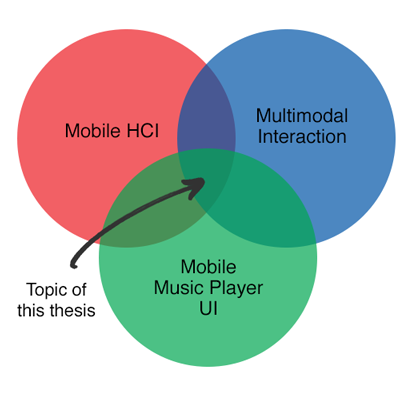
\includegraphics[width=0.5\textwidth,height=\textheight,keepaspectratio]{./Figures/venn.png}
		\rule{35em}{0.5pt}
	\caption[Venn diagram]{Thesis topic position}
	\label{fig:venn}
\end{figure}


\section{Mobile Human Computer Interaction}
The term "Human Computer Interaction" involves the study, planning and design of the interaction between human and computers \cite{card_psychology_1983}. This term supports a view both from the computer and from the human perspective. From a computer perspective in the mobile HCI community challenges like short battery life, network volatility, limited memory/processing power typically arise and specific system design patterns have been designed to handle this \cite{roth_patterns_2002}. From a mobile human perspective the term "nomadic computing" can be used where the main requirements for such a system is defined as providing capabilities and services to the nomad as he/she moves from place to place in a transparent, integrated and convenient way \cite{sawhney_nomadic_2000}.

% this project
In this project a mobile music player for cyclists is developed so the focus will be on the interaction between a user and device while the user is in motion. This kind of interaction has also been defined as "interaction in motion" \cite{marshall_mobile_2013}.

\subsection{Interaction in motion}
\label{sec:interactioninmotion}
According to Marshall and Tennent \cite{marshall_mobile_2013} mobile interaction does not exist as most mobile systems are designed for active interaction when a user is standing still dedicating his/her full attention to the device. Specific mobile systems should instead allow the user to interact while in motion e.g. driving, running or in this thesis case biking. To develop such kind of system specific challenges needs to be solved and Marshall and Tennent have classified these into four categories \cite{marshall_mobile_2013}:

\begin{description}
\item[Cognitive Load]
Essentially this concept is decribed as a person only being able to pay attention to a certain amount of things at once. When this limit is reached the person stops paying attention to other things. This means that even though a person is able physically to sense, hear or feel multiple interaction tasks, it may not be possible to attend to all these tasks at the same time.

% from the systems point of view
Depending on the mobile interactive system this cognitive load can change over time. If a person is forced to actively attend or respond to the system the cognitive load is increased while a passive output from the system can decrease the cogntitive load. Also the content of information being addressed to the person can affect the cognitive load e.g. when making phone calls a discussion with an interviewer is less distracting than performing a simple memory test \cite{nunes_cognitive_2002}.

% environment
The cognitive load can also depend on environmental factors e.g. the movement activity in which the user is performing. Physical challenges e.g. walking a plane ground vs. climbing stairs can effect the mental demand of the user i.e. increase the cognitive load.

\item[Physical Constraints]
Mobile systems and user movement activities can both add constraints on the body position which could lead to a conflict making it hard or even impossible to interact. E.g. as mentioned earlier biking physically needs the hands for steering and eyes on the road while both of these body parts are used in the traditional smartphone interaction form (eyes on the screen, hands for touch gestures). This has been identified to be a major barrier to the use of mobile system whilst moving \cite{pielot_pocketmenu:_2012}.

\item[Terrain]
The terrain is described by the enviroment around a person while moving and interacting. Studies have shown that while running and interacting the terrain over which a person was running made a big difference in the interaction experience and the ability to concentrate on the output of the system \cite{marshall_using_2011}.

Physical terrain can be dynamic i.e. it can change over time while moving around different environments e.g. road obsticles, traffic, light level, rain, sound, etc. This could not only affect the user interaction experience but also the electronic device e.g. water or extreme cold/heat.

\item[Other people]
This class relates to other people during a interaction. For example in a crowded place the user needs to take care of people passing by while interacting with the mobile device. Or When biking the user needs to take care of people making an overhaul, communicating or waving back to a friend on the sidewalk. The social aspect of the environment a person is in can also have an impact on the device interaction e.g. in a quiet place a person would probably not use speech commands to interact with a device as this would be socially impolite.
\end{description}


\section{Multimodal interaction}
While the previous section was about planning and designing the interaction between humans and computers, this section describes how the actual information between a human and computer could be exchanged. 

\subsection{Modality definition and use}
Bolt was one of the first to define the term modality in a study where speech and gesture in combination was used as input to a system \cite{bolt_put-that-there:_1980}. Modalities has something to do with the mode of communication according to the human senses and input devices activated by humans \cite{jaimes_multimodal_2007,tzovaras_dimitrios_multimodal_2008}. The human senses are \textit{sight}, \textit{touch}, \textit{hearing}, \textit{smell} and \textit{taste}. Input modalities of many computer input devices can then be considered to correspond to these senses e.g. cameras (\textit{sight}), haptic sensors (\textit{touch}), microphones (\textit{hearing}). While the term multimodal has been used in many different contexts and disciplines this thesis will focus on Tzovaras definition: \textit{"During interaction, the user produces input modalities to the system and the system produces output modalities to the user. A multimodal interactive system is a system that uses at least two different modalities for input and/or output. And a unimodal system is a system which uses the same single modality for input and output"} \cite{tzovaras_dimitrios_multimodal_2008}. The word input is defined by \cite{jaimes_multimodal_2007} to be of great importance as in practice most interactions take place using multiple modalities e.g. typing a keyboard (\textit{touch}) while looking at the keys or screen (\textit{sight}) to see whats being typed.

% modality combinations
Modalities can be used in combination with each other in different ways. In the "Put that there" system \cite{bolt_put-that-there:_1980} modalities are used in a complementary combination as the user can point the items on a large display and select or move them by vocal commands. In this case gestures and speech modalities are strengthening each other. In other cases modalities can act simultaneously giving different kind of information about the same feature e.g. visual and acoustic alarms in a building. Both these modality combinations have no unexpected implications in terms of the information that needs to be delivered. Either the information can only be gained in one way (complimentary approach) or the user can choose which way to gain the information (simultaneous approach). A case where modality combinations can have unexpected behaviour is when a modality is replaced with another to deliver the exact same information e.g. gaining an overview of a music collection would seem unnatural with voice commands compaired to a visual overview. This causes a non-linear effect and introduce more complexity to the interaction system.

\subsection{Multimodality in mobile systems}
As mentioned in \ref{sec:interactioninmotion} interacting with a device in motion introduces different challenges like environmental and human attention factors. This could imply that for some mobile situations certain multimodal interaction types would fit better than others. Much of the interfaces work especially in wearable computing tends to focus on visual headmounted displays \cite{barfield_fundamentals_2000} e.g. Google Project Glass. But not only does visual displays occupy the users visual attention, they can also be obtrusive and hard to use in bright daylight \cite{geelhoed_safety_2000}. Visual displays power consumption is must often also high i.e. they drain a mobile device battery and they are expensive.

% Eyes-free interfaces term
Several work on both audio \cite{kajastila_eyes-free_2013,bonner_no-look_2010,brewster_multimodaleyes-freeinteraction_2003,zhao_earpod:_2007,vazquez-alvarez_eyes-free_2011} and haptic \cite{pasquero_haptic_2011,pielot_tactile_2011} interfaces use the term eyes-free which refers to controlling the state of a system without visual attention. This kind of interaction has shown to be desirable in some mobile situations \cite{oakley_designing_2007,yi_exploring_2012} and even improve efficiency compaired to traditional visual displays \cite{zhao_earpod:_2007}. Eyes-free interfaces can keep the users visual attention on the road while driving \cite{sodnik_user_2008} or walking around in the city \cite{vazquez-alvarez_eyes-free_2011}. It should be taken into account though that just because information comes from a different modality that the one in use, it doesn't mean that the user is not distracted cognitively as described in \ref{sec:interactioninmotion}.

% Eyes-free modalities focus
Eye-free interfaces are not limited to specific modalities. As mentioned in \ref{sec:alternativemusicuis} input modalities like speech, gesture and touch combined with audio or haptic feedback can "detach" the eyes from the interface. As this project focus is on a concrete mobile scenario i.e. biking - not only should the interface be eyes-free but also "hands-free" (as biking requires steering). To avoid the use of \textit{sight} and \textit{touch} human senses the proposed interface includes head gestures as input and audio as output.

\subsection{Head gestures as input modality}

% intro - alternative head tracking methods
There exists different kinds of approaches when it comes to controlling a system with head gestures. Using cameras it is possible to effectively track head movements via facial recognition \cite{morimoto_recognition_1996} and gaze tracking makes it possible to control an object by fixating the eyes on that object while moving the head \cite{vspakov_enhanced_2012}. Thus these techniques do not require any hardware sensors e.g. accelerometer and gyroscope but in return a camera placed in front of the user. Although this method has been conducted for mobile devices \cite{mardanbegi_eye-based_2012} the setup will still require the eyes in a combination with head gestures as an input modality.

Instead sensor based detection of head movements could be used e.g. accelerometer and gyroscope. Both Brewster et. al \cite{brewster_multimodaleyes-freeinteraction_2003} and Park et. al \cite{park_gaze-directed_2011} have evaluated systems using this kind of sensor based head gesture input. In these systems custom wearable hardware was built to physically place sensors on the users head but today this kind of hardware is actually accessible \cite{gn_store_nord_intelligent_2013}. Headsets are shown in fig. \ref{fig:headsets}.

\begin{figure}[htbp]
	\centering
		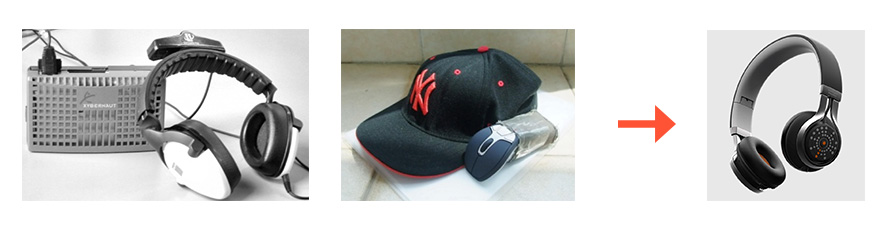
\includegraphics[width=\textwidth,height=\textheight,keepaspectratio]{./Figures/headset-development.jpg}
		\rule{35em}{0.5pt}
	\caption[Headset Development]{Wearable interfaces used before (left \cite{brewster_multimodaleyes-freeinteraction_2003} and middle \cite{park_gaze-directed_2011}) compaired with todays accessible interface (right \cite{gn_store_nord_intelligent_2013}).}
	\label{fig:headsets}
\end{figure}

With this interface it is possible to detect not only the head rotation (gyroscope) but also the acceleration (accelerometer) when the head is moving. There exists advanced algorithms for recognizing motion gestures \cite{lu_head_2005, kratz_combining_2013, akl_accelerometer-based_2010} but this project will use a simple Dynamic Time Warping algorithm \cite{meinard_muller_information_2007} as the gestures used are short and simple e.g. nodding or shaking the head and the focus is not on optimizing and precisioning the gestures.

\subsection{Audio as output modality}
\label{sec:audiomodality}
Replacing visual with audio output has shown to have a positive effect when interacting in motion. Brewster showed, by compairing visual and audio feedback when pushing buttons on the same GUI, that it was difficult for users to devote all their visual attention to an interface while walking, running og driving and that the interaction workload decreased with audio feedback \cite{brewster_overcoming_2002}.

% Speech vs Non-speech audio
Audio output can in general be divided in two ways \cite{rocchesso_sounding_2003}:
\begin{description}
\item{1: \textit{Speech audio}}, can use a computer recorded human voice like in a guided audio tour for tourists.
\item{2: \textit{Non-speech audio}}, can be used for presenting more complex information e.g. music or other sounds.
\end{description}

Work has shown that non-speech audio is effective in improving the interaction in mobile environments \cite{pirhonen_gestural_2002, sawhney_nomadic_2000}.

When presenting the audio it's important to consider the attention which is required by the user while this can have a great impact on the cognitive load. Brewster et. al \cite{vazquez-alvarez_eyes-free_2011} presents two kinds of attention-tasks:

\begin{description}
\item{1: \textit{Selective-attention task}}, presenting multiple audio streams the user selectively choose which one to assign the attention e.g. listening to a voicemail while listening to a music track. This results in a lower cognitive load.

\item{2: \textit{Divided-attention task}}, in this case the user is forced to respond to each audio stream presented e.g. talking over the phone while interacting with a calendar using a audio menu. The attention gets divided and result in a higher cognitive load.
\end{description}

In this project multiple audio sources (music tracks) are presented for the user at the same time but none of them requires a respond i.e. the focus is on selective-attention tasks.


\subsection{Spatial audio interaction}
This section describes how the before mentioned modalities - head gestures input and audio output can be used for interaction with the enforcement of spatial audio.

% intro - what is spatial audio, HRTF
Spatial audio or 3D audio allows a sound source to appear as if it is coming from anywhere in space around a listener \cite{begault_3dd_1994}. This can be achieved by using HRTF (Head Related Transfer Function). HRTF attempts to model the frequency modulations of a sound entering the human ear from a given direction and is implemented in many soundcards today.

% Advantages refs
Spatial audio has shown to be effective in several aspects. William W. Gaver, a pioneer in audio interfaces, has explored the intuitiveness of presenting complex information to users in the form of audio \cite{gaver_sonicfinder:_1989}. Similarly Graham explores the advantages in reaction time when using "auditory icons" \cite{graham_use_1999}. Gaver presents the use of spatial sound icons \cite{gaver_auditory_1986}. In doing so, he draws forward the unutilized potential of creating natural interaction through spatial audio.

% Multiple sound sources, cognitive load effect
Previous research has also shown that spatial audio is a successful technique for segregating multiple audio streams \cite{schmandt_audiostreamer:_1995, walker_spatial_2000}. Brewster et. al \cite{vazquez-alvarez_eyes-free_2011} shows in a study that when users must be able to direct their attention selectively to each individual audio stream representing a task (selective-attention task) - spatial audio had a great effect. In this case the cognitive load was kept low as described in \ref{sec:audiomodality}.

% Audio menus

% 1D/2D - my defintion

% Maybe Intelligent Headset (Headset Interface)


\section{Mobile Audio User Interfaces}
This section describes the systems that are most related to this project. Alternative mobile music player user interfaces are presented first - alternative in the sense that the interaction form is different from the traditional way (touch input and visual output). Also other systems - not music related - are presented. These systems uses an interaction form that is close to the desired one in this project. Finally all systems properties are compaired and visualised in a table.

\subsection{Alternative music player UI's}
\label{sec:alternativemusicuis}
There exists music player interfaces that attempts to use eyes-free interaction when listening to music on the go and they are presented in this section.

% headset controller
Headset music controllers are physical buttons attached to the wire between headset and device. This controller typically includes play, stop, next track, previous track and volume buttons. Such a controller would require only one hand from the user to interact with a music application. This kind of interaction though assumes the user has created a playlist and knows in which order the tracks follows to navigate efficiently to the wanted track. Also this kind of interaction menu is 1-dimensional in the sense that numbers have to be placed in a sequence missing the opportunity to go into a submenu e.g. an album of an artist. It should also be taken into account that although only using one hand for interaction this could still create challenges e.g. when steering or hitting the breakes while biking could require both hands on the steering.

[IMAGE (headset music controller)]

% voice recognition
Voice recognition could also be used for navigating a music application \cite{stewart_boling_voice_2013}. In this application example the user could request simple commands like play, stop, next/previous track and queue. Voice recognition however introduces accuracy and stability challenges especially in mobile noisy environments. At the same time speech commands are limited - it would introduce even more complexity if the system should be able to interpret detailed commands e.g. an artist name or even a track title.

% other alternatives
Other more alternative music player interaction modes also exists using motion sensors. A system that use foot gestures for changing music track has been developed and shows a highly efficient way of interacting while running \cite{smus_running_2010}. Another system also using gesture recognition controls a music player by placing a device on different body parts e.g. placing it by side of the head while nodding changes the music track \cite{strachan_bodyspace_2007}.

[IMAGES (leg shifting track + body parts interaction)]

All these systems have in common that they avoid the users visual attention but they are all limited to basic controls such as play, stop, next/previous track, volume up/down.

\subsection{Spatial audio interaction systems}
Other systems - though not all mobile music players - uses a spatial audio interaction form and they can contribute to this projects final system in form of e.g. menu and audio design, navigation, etc.

% 1, Multimodal'eyes-free'interaction techniques for wearable devices
Brewster et. al \cite{brewster_multimodaleyes-freeinteraction_2003} evaluated to kinds of eyes-free wearable systems. The first system includes a 3D audio radial pie menu 

Brewster et al. showed that novel interaction techniques based on sound and gesture can significantly improve the usability of a wearable device in particular under "eyes-free" mobile conditions and that head gestures was a successful interaction technique with egocentric sounds the most effective \cite{brewster_multimodaleyes-freeinteraction_2003}.

% 2, Gaze-Directed Hands-Free Interface for Mobile Interaction
Park et al. also experimented, using head gesture input and aural output, with 1D and 2D menu interfaces \cite{park_gaze-directed_2011}.

% 3, Interaction with eyes-free and gestural interfaces
Kajastila and Lokki has done a user study comparing auditory and visual menus controlled by the same free-hand gestures where the majority of the participants felt that an auditory circular menu was faster than a visual based menu \cite{kajastila_interaction_2013}.

% 4, Gestural and Audio Metaphors As a Means of Control for Mobile Devices
Touch gesture and non-speech audio as ways to improve the user interface of a mobile music player \cite{pirhonen_gestural_2002}.

\subsection{Systems properties overview}
For this project specific properties of the system are required. Related systems that contains these properties can be valuable input for this project. To give an overview - these properties are presented in table \ref{tab:related}.

\begin{table}[h] 
\caption{Related works properties comparison} % title name of the table 
%\centering % centering table

% Properties
% - In-motion interaction
% - Output modality
% - Input modality (Head, foot, hand)
% - Menu depth (1D, 2D)
% - Using accessible hardware
% - Controlling music application
% - 1-1 evaluation against real world application

\begin{tabular}{L{4cm}C{2cm}C{2cm}C{2cm}C{2cm}} \toprule
    Properties & System 1 & System 2 & System 3 & System 4 \\ \midrule
    In-motion interaction   & + & + & - & - \\
    \\
	Output modality \\ %\midrule
	\\
	Input modality (Head, foot, hand) \\
	\\
	Menu depth (1D, 2D) \\
	\\
	Using accessible hardware \\
	\\
	Controlling music application \\
	\\
	1-1 evaluation against real world application \\ \bottomrule
\end{tabular}

\label{tab:related} 
\end{table}








 % Background

\lhead{\emph{Design}}
\chapter{Design}
\label{sec:design}
In this chapter the design of the system is described. Although we have decided from the beginning to design a system based on head gestures and audio modalities, we will still discuss how alternative modalities based on existing systems and related research from chapter \ref{sec:relatedwork} would fit in a biking scenario. This will give a better insight of the importance of modality choice - the benefits and tradeoffs - when designing systems for interaction in-motion. Also the related systems could contribute to the design of specific features for our final system. This is part of the design rationale and covers the first part of this chapter. In the second part the final system design is presented.


\section{Design Rationale}
% Intro
Before choosing a design for a system different factors needs to be considered e.g. the reasons behind the design decisions and the justification for it; other design alternatives considerations and the tradeoffs when choosing a design over another; the argumentation that lead to the design.

% Ubicomp challenges
When designing for ubicomp new aspects needs to be taken into consideration which increase the complexity of the system e.g. different devices, mobile users and changing environment and context \cite{barfield_fundamentals_2000}. Also we note that we are not only designing user interfaces but also the interactions between a user and the system through artifacts embedded in the environment \cite{beaudouin-lafon_designing_2004}. Furthermore it should be taken into account whether the interaction happens while the user is in motion as this introduces even more complexity as decribed earlier in section \ref{sec:interactioninmotion}.

In this project we have defined the following requirements of the system: A user should navigate a music player while biking. In other words we have a user interacting with artifacts, in order to explore and select music tracks, while biking in a traffic environment implying user awareness of road conditions, cars, other bikers, etc.

As a consequence of these requirements, we will in the next sections discuss the constraints emitting from a scenario like that and how modality combinations could fit in the design of such a system. This will result in a discussion on related systems, that uses the audio modality as interaction form. Last we will delve further into specific related audio interfaces and look at different auditory menu designs.

\subsection{Biking scenario constraints}
% intro, physical and mental constraints
Several constraints emerge from a humans capabilities to interact with a system while biking, both physically and mentally. Seen from a physical perspective the person riding the bike needs to have both hands on the handlebars in order to dodge any sudden obstructions e.g. an inattentive car. For the same reasons, and more importantly, the persons eyes needs to focus on the road. The latter is of more importance from the fact that people can not easily divide their visual attention between tasks \cite{brewster_overcoming_2002} but two hands can work independently from each other, dedicating one for steering and one for the interface. This does not mean that one hand can steer a bike perfectly - this is subjective, and we must assume that both hands for steering is preferable. Lastly biking requires the legs/feed on the pedals to move forward. From a mental perspective biking is heavily depending on the users attention or perceptual load first of all to navigate the road but more importantly to keep the ability to react to traffical events. This perceptual load is complemented by the cognitive load which can increase in a very busy traffical biking scenarios and depends on the users ability to handle such scenarios.

From a system perspective a biking scenario also implies constraints. First of all interaction with the system should preferably go through some kind of wearable device or at least something easy installable hardware that could be attached to the bike. The system also needs to optimize handling of unintentional interaction during biking e.g. motion gestures when riding a bumpy road. Secondly and most important the system needs to aim for minimizing the workload required by the user - every added feature should be considered i.e. every interaction task should be considering conducted while biking. Also the content presented to the user should be considered in terms of the interaction modality being used e.g. in a visual music player interface artist/track information and a lot of navigation possibilities might be good but if the same information and functionality were to provided via audio this would cause a non-linear effect and add too much complexity to the system.

\subsection{Modalities reasoning}

% HMD, Gaze tracking
\textbf{Visual challenges}

A headmounted visual display like Google Glass would give total hands-freeness when biking but as mentioned in \ref{sec:interactioninmotion} such displays can be hard and obtrusive to use in bright daylight. Also such interface still would require the visual attention from the user \cite{geelhoed_safety_2000}, although the user would not have to change head direction while biking (like when looking down on a traditional stop-to-interact interface). Same arguments follows with a gaze tracking solution. Also such a solution could require some kind of installation on the bike e.g. a camera attached to the handlebars for tracking the eye. Mobile solutions exists \cite{mardanbegi_eye-based_2012} but this will still imply the user to look at the device, and probably hold the device i.e. occupying one hand, while interacting. However the benefit with using visual displays like the headmounted displays in our scenario is, that it's possible to keep the rich visual experience of exploring music tracks before selecting them - information could be linearly translated from the stop-to-interact music player interfaces. It can be argued though, that the experience is not as rich when biking in a traffic environment where attention is divided.

Studies on multimodal interaction \cite{zhao_shared_2013} have shown that when humans needs to attend a physical visual task and a virtual task at the same time (dual task situation) - they found it significantly distractive to attend to the virtual task in a visual way. Instead audio has shown to be less distractive. The biking while interacting scenario can easily be translated into such a dual task where the physical task is to attend to the road and traffic and virtual task is to explore and select music tracks. Inspired from this and from other studies showing that audio can improve usability with mobile devices in eyes-free mobile conditions \cite{brewster_multimodaleyes-freeinteraction_2003}, systems designs that uses audio modalities should be considered instead.

% Audio interfaces/related systems
\textbf{Audio modality combinations}

% voice recognition
Using audio both as input and output modality would imply some kind of voice recognition system like the Google Search voice command system for Android mentioned in section \ref{sec:alternativemusicuis}. A good thing about this system is that the hardware requirements are minimal - it would work on all devices supporting Android and with all kinds of headsets. From a physical and workload demanding perspective this could work in a biking scenario e.g. a user would have to pick out the phone (maybe from the pocket) and then place it near the mouth and give the command. The visual attention would still be on the traffical surroundings although picking out the phone could need some attention. By using a headset controller with a mic this possible "hand attention problem" could be avoided. This interface however have some challenges \cite{sawhney_nomadic_2000} especially in noisy environments, where voice commands can be hard to recognize by the system, making it tedious and frustrating for the user to keep repeating the command. This frustration and also that the user is doing a physical activity like biking (increasing heart rate), can change the voice and affect the systems recognition abilities. At the same time these commands are limited i.e. navigation is limited. Too many commands would add heavy complexity to the system e.g. imagine a stop-to-interact music player interface like Spotify to translate just 10 of their navigation features to a voice command system. This will create a non-linear effect i.e. the user will have a hard time just remembering the commands and could get lost quickly in the navigation.

% touch based
Touch and audio based interfaces also suffers from limited navigation controls. Todays headset music controllers however fits well in a biking scenario. Although using one hand while biking to navigate the interface, the time it takes to push a button is short i.e. reducing the time where the bike is controlled with one hand. This short navigation maneuver is also due to the limited possible interface controls. Similar to these head controllers are the touch based interfaces that uses touch screens \cite{pielot_pocketmenu:_2012, pirhonen_gestural_2002} - controlled from the pocket. These interfaces however uses more advanced output modalities e.g. audio/tactile simultanous modalities (PocketMenu) and spatial audio feedback, which potentially could be used for richer exploration of menu items but also possibly increase complexity i.e. making it a harder cognitive task. Considering these advanced output modalities spatial audio has shown to be able to present complex information \cite{bronkhorst_cocktail_2000, gaver_sonicfinder:_1989} while keeping the human cognitive load down \cite{vazquez-alvarez_eyes-free_2011} and in combination with gesture input modalities, it was used effectively when navigating an interface in eyes-free mobile conditions. 

Considering combining spatial audio output with a motion gesture input modality, possible available human body parts when biking could be hands (implies biking with one hand) or the head. Although feet as a modality input were evaluated in a running scenario with good results \cite{smus_running_2010}, it would be awkward when biking would require both feet on the pedals to keep moving. Kajastilas free-hand gestures \cite{kajastila_interaction_2013} would imply the same hand interaction challenges discussed above but also a camera installed on the bike to detect the movements. Sensors could be used instead but would require some artefact installed on the hand. Instead it would be more appropriate to install sensors into a headset and use head movements as input modality like \cite{park_gaze-directed_2011, brewster_multimodaleyes-freeinteraction_2003} as this would not add any additional artefacts to the system. When using head gestures it would still be possible to keep the eyes on the road, assuming the head rotation is not too big. Also the human head itself is physically constrained in that it can be rotated 140 degress for shaking and 100 degrees for nodding \cite{lopresti_neck_2000} which should be taken into consideration when designing the auditory menu. Also when biking motion gesture detections could be unintentionally activated e.g. an accelerometer sensor value increases when moving forward.

With the chosen modalities of head gestures and spatial audio in mind we will next compaire auditory menu designs that uses these modalities and discuss their customizability in a music listening biking scenario.

\subsection{Auditory menus}
To achieve the first goal of this thesis that is, to design a mobile music player interface based on head gestures and 3D audio that allows a user to explore and select music tracks, we have discussed the interaction scenario constraints above and the suitability of modality choices, but we also need to consider the minimum requirements of the system: The exploration and selection of music tracks. This is more related to the content of the system and how it is presented. To compete with existing "stop-to-interact" music player interfaces in terms of this, we need to translate as much of the visual information into audio feedback without causing any non-linear effects.

One advantage with using a multimodality combination of head gestures and spatial audio is that it can provide natural interaction \cite{gaver_auditory_1986} i.e. hearing sounds as we would normally do in the real world in relation to head direction. Another advantage with spatial audio is that it can enable the "cocktail party effect" \cite{bronkhorst_cocktail_2000} i.e. people can segregate multiple simultanous playing sounds. Imagining if exploring simultanous playing music tracks is feasible, that could provide a rich exploration factor to our music player interface - allowing the user to hear tracks before selecting them.

Although Park et. al \cite{park_gaze-directed_2011} showed good results with a 2D grid menu it is hard to localize vertically positioned sounds compaired if they were aligned horizontally - especially if they play simultanously. A circular egocentric menu layout showed the best evaluation results in the head gesture system by Brewster et. al \cite{brewster_multimodaleyes-freeinteraction_2003} but they were limited to 4 sound items because of head movement constraints (a nod in 45 degrees is hard for a human to conduct). Although same study showed that an exocentric layout were slower it would give a more natural selection (directing the head against an item and selecting it) and provide the opportunity for more than 4 sound items.


\section{Spatial Music Menu}
This section contains a description of the system design. The physical design of the system assumes artefacts in form of a headset, which can detect head gestures by using built-in motion sensors and deliver 3D audio feedback, that communicates with a mobile device put in the users pocket during biking.

\begin{figure}[t]
	\centering
		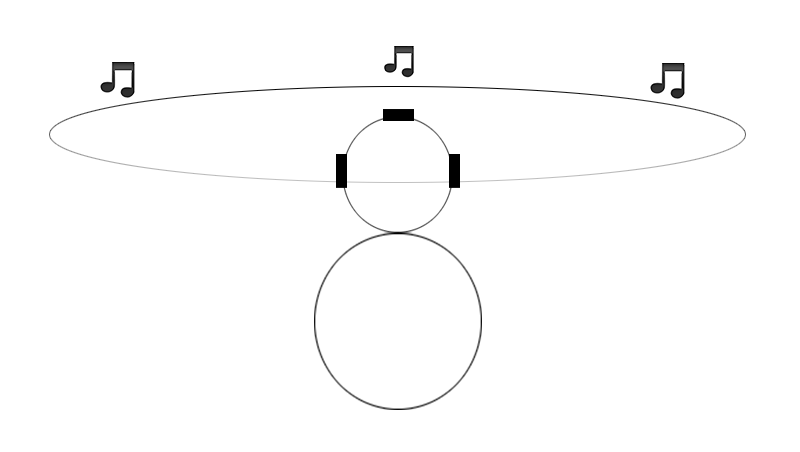
\includegraphics[width=0.6\textwidth,height=\textheight,keepaspectratio]{./Figures/sounddesign.png}
		\rule{35em}{0.5pt}
	\caption[Soundscape Design]{Soundscape Design - Visualising how the circular auditory menu surrounds a person (viewed from the persons back)}
	\label{fig:sounddesign}
\end{figure}

\subsection{Soundscape design}
Non-speech sound items (music tracks) are layed out in a horizontal circular way within 140 degrees in front of the user, see figure \ref{fig:sounddesign}. The number of music tracks are spatially positioned and are playing simultanously. The menu uses exocentric interaction - by turning the head towards a music track, it will move in the center of the users front audio space. We conducted a small pilot study where 2 kinds of design were tested. The two designs can best be described by imagining a carousel turning, while different music concerts play around it. In the first design the user stands in the center of the carousel looking out and in the second the user stands on the edge of the carousel looking out. These two interaction modes are illustrated in figure \ref{fig:interactionmodes}.

\begin{figure}[t]
	\centering
		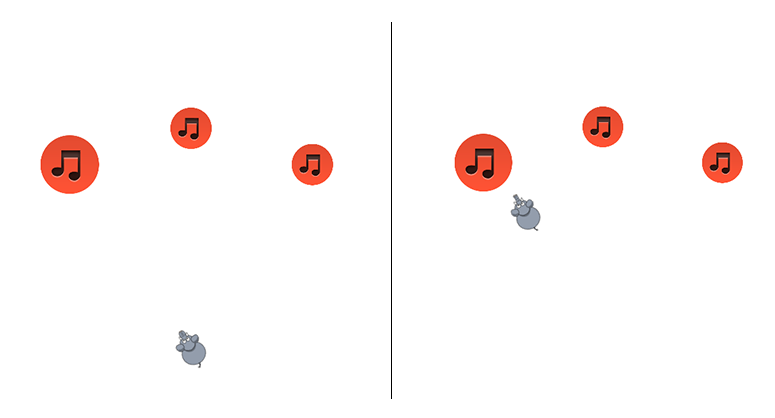
\includegraphics[width=0.9\textwidth,height=\textheight,keepaspectratio]{./Figures/interactionmodes.png}
		\rule{35em}{0.5pt}
	\caption[Interaction modes]{The system consists of two different interaction modes - with (to the right) and without (to the left) zoom feature. The user is illustrated by an elephant looking at the sound items.}
	\label{fig:interactionmodes}
\end{figure}

The purpose of the pilot study was to give qualitative feedback and specify appropriate parameters like max number of simultanous playing music tracks, the preferred degree for head rotation and the distance between the user and the music items. Although not neccesary for the final design, we developed a hifi-prototype \cite{benyon_designing_2010} that visualised the actual soundscape design. This envisionment technique gave the users in the pilot study a quicker and better understanding of the design. Figure \ref{fig:pilotstudy} shows a user testing the design and the hifi-prototype.

\begin{figure}[b]
	\centering
		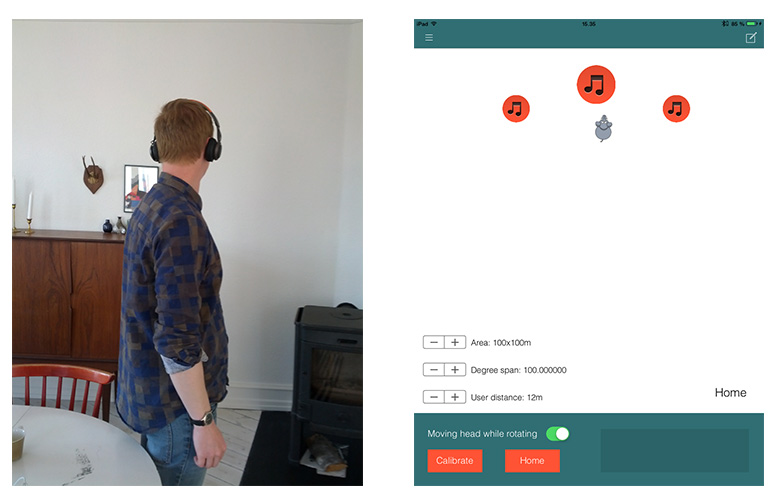
\includegraphics[width=0.9\textwidth,height=\textheight,keepaspectratio]{./Figures/pilotstudy.jpg}
		\rule{35em}{0.5pt}
	\caption[Pilot study]{Pilot study showing a user testing the design and the visual prototype.}
	\label{fig:pilotstudy}
\end{figure}

The pilot study consisted of 5 participants, 4 males and 1 female. The music tracks used in the test were added by the users to make sure they knew the tracks. The experiment were conducted by observation and semi-structured interviewing \cite{benyon_designing_2010}. Both interaction modes were tested by starting laying out 3 sound items and then adding 1 item iteratively until the user found it too hard to recognize the music tracks. Distance and head rotation parameters were adjusted to match the user preferences every time sound items were added. The users preferred the interaction mode with zoom effect and they felt comfortable with 6-8 simultanous playing music tracks compaired to the other mode where \textgreater 4 simultanous music tracks were hard to segregate. Users preferred a smaller head rotation degree with the zoom effect of 80-100 degrees compaired to the other mode where 120-140 degrees were preferred. The feedback results are shown in table \ref{tab:pilotresults}.

\begin{table}[t] 
\scriptsize
\centering
\caption{Pilot study feedback} % title name of the table 
%\centering % centering table
\begin{tabular}{L{3cm}C{3cm}C{3cm}} \toprule
	 & Direction based & Direction based with zoom effect \\ \midrule
    Max number of music tracks   & 3-5 & 6-8 \\
    \\
    Preferred head rotation degree   & 120-140 & 80-100 \\ \bottomrule
\end{tabular}

\label{tab:pilotresults} 
\end{table}

\subsection{Navigation}
The menu was designed with a 2 level exploring part that utilizes the soundscape design and a final level for playing the music track (simple playback). The idea is that the exploring starts by selecting an artist (HOME), then moving up a level to select a track from that artist (ALBUM) and then finally playing it (PLAYING TRACK). This menu hierachy (reversed) is illustrated in figure \ref{fig:navigation}.

\begin{figure}[b]
	\centering
		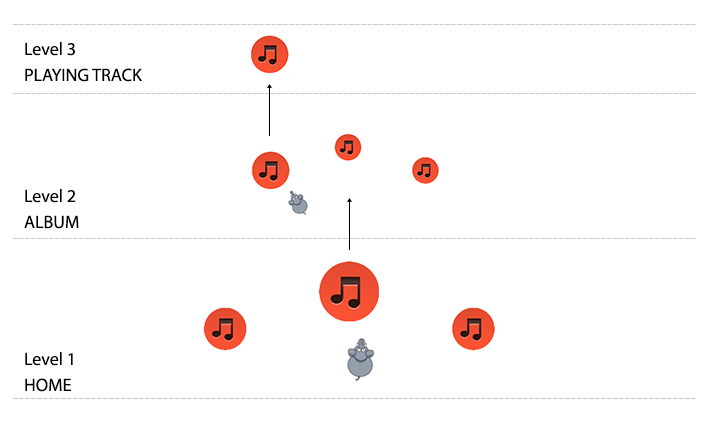
\includegraphics[width=0.8\textwidth,height=\textheight,keepaspectratio]{./Figures/navigation.png}
		\rule{35em}{0.5pt}
	\caption[Menu Hierachy]{The menu consists of 2 exploring levels and 1 level for playing track.}
	\label{fig:navigation}
\end{figure}

To navigate between levels simple head gestures were designed: A forward nod for going up one level, a backward nod for going back one level and a right sideways nod for activating the menu. Activating the menu would be the case where a music track is playing and the user wish to change track - it will take the user to the HOME level. When entering a level, audio feedback is given in form of speech recorded sounds telling what level the user is in e.g. "Home", "Album" and "Playing track". These head gestures and the ability to navigate between menu levels were evaluated in a second part of the pilot study mentioned above. Participants started by recording the three gestures (3x3) to get some training data. Then the participants simply tried to choose tracks by navigating between levels using the gestures. The system seemed to react to undesired gestures (false positives) when participants were rotating the head which affected the navigation experience negatively. Backward and sideways nods were removed and instead to go up one level or to activate the menu a simple push on a button on the headset were introduced. This helped in several ways - the user only needed to focus on 1 gesture which they also reported was the easiest gesture to conduct. For the systems point of view the nod is the most important gesture in that it is the actual selection of an item. We assume users most of the time to select the desired music track, and therefore going back a level would at least not be as neccesary as selecting i.e. we would not expect a lot of button push activity. Same theory goes for activating, this will be a 1 time push for every time the user wishes to change track. An accuracy test were conducted for nod selections by observing a user and the system response registering true postitives (nod performed and detected), true negatives (nod performed but not detected) and false positives (nod detected but not performed). The participant simply performed nods while turning the head in different directions in between and every event, whether it was a performed nod or a detected nod by the system, were noted down. Table \ref{tab:accuracytest} shows the results of 200 registered events - 100 from two different users.

\begin{table}[h] 
\scriptsize
\centering
\caption{Nod gesture accuracy test} % title name of the table 
%\centering % centering table
\begin{tabular}{|C{3cm}|C{3cm}|C{3cm}|}
	\hline
	True Positive & True Negative & False Positive \\ \hline
    163 & 35 & 2 \\ \hline
\end{tabular}
\label{tab:accuracytest} 
\end{table}

163 of 200 events were executed correctly so we end up with an accuracy of $\sim$ 82\%. Decreasing the number of gestures had the desired effect and the false positives were reduced to only 2 detections during the 200 events.




















% OLD - Use some parts here and move some to introduction method section


%The design is based on the following parameters: 

%\begin{itemize}
%\item Simultanous sounds (music tracks) spatially positioned
%\item Horizontal circular menu layout with music tracks as menu items
%\item Non-speech sound items in form of music tracks
%\item Simple speech sound feedback indicating menu level
%\end{itemize}

%- Music, strength of recognizing artist/track through listening vs seeing the text on a screen
%- Horizontal argument
%- Two menu interaction modes, distance/
%- Selective attention task
%- Simultanous sounds, exploring, cocktail party effect argument
%- Experimental design, sounds perceived, zoom effect, user should detect sound direction (which track)

% Horiontal alignment

% Circular

% non-speech sound

% selective-attention

% exocentric

% Head gestures, nod=yes




\begin{comment}

This chapter first explains the design methods used and the most important design activities and choices made in the design process. Based on this process the final prototype design is presented at the end of the chapter.

\section{Design model and methods}
In this section the model used for designing the final prototype is presented including the different techniques used throughout the design process.

The related works conducts the foundations for an early first prototype. This prototype will then go through an iterative design process, taking a user centered approach. This will enable specifications to emerge during the process and these learnings and modifications will result in new experiments and prototypes. This iterative design model is illustrated in figure \ref{fig:iterative}.

\begin{figure}[t]
	\centering
		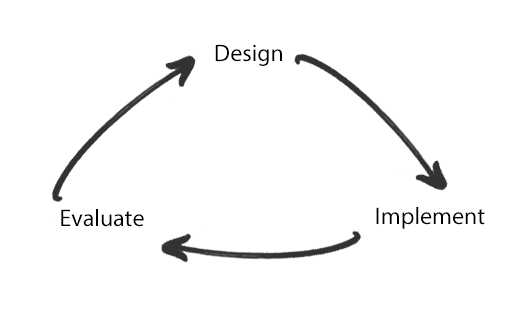
\includegraphics[width=0.6\textwidth,height=\textheight,keepaspectratio]{./Figures/iterative.png}
		\rule{35em}{0.5pt}
	\caption[Iterative Design Model]{Iterative Design Model}
	\label{fig:iterative}
\end{figure}

\subsection{Envisionment}
One of the goals with the final system is that it should be eyes-free i.e. the user should not depend on a visual screen UI at the end. Despite this goal, the use of a screen to visualize e.g. a virtual menu, can be helpful in the design process. This will enable test users to get a quicker and better understanding of how the interaction works. In this design process a mobile device screen will be used for envisionment - this is also called a hifi prototype or software prototype \cite{benyon_designing_2010}.

More concretely audio sources and the users head position including rotation will be mapped visually to a screen dynamically during user interaction. An example of this screen is shown in figure ?

\section{Design process}
This section starts out by describing the first experimental prototype design inspired from previous research work and then each iteration including user feedback and design changes and experiments. More specifically the design completed 2 iterations before the final prototype design.

\subsection{Initial prototype design considerations}
Before we started to reason about initial design choices we started out by defining what the system actually needed in order to evaluate and revise the hypothesis from the problem statement.

% intro, track exploring
First of all we wanted the system to be able to play music. This is in itself a trivial task but as we the same time wanted to control the system only with with head gestures and audio output a traditional music player includes too many options e.g. play, pause, stop, next/previous, volume, equalizer, track exploring, etc for the scope of this thesis. All the alternative music players mentioned in chapter \ref{sec:relatedwork} is limited to simple commands like play, stop, next/previous and volume. Taking it a step further we wanted to evaluate the track exploring part i.e. navigating to a preferred track and playing it. This made et clear that some kind of auditory menu with tracks as menu items was needed and although not music players the related systems from chapter \ref{sec:relatedwork} using auditory menus could inspire to an intital menu design.

% Auditory menu, exocentric, head rotation constraints
When looking at the different related auditory menu designs we needed to find a design that fitted into the context of the user activity i.e. biking and also user interaction modality. E.g. in a biking scenario the user should have eyes on the road thereby constraining the head rotation. Park et. al \cite{park_gaze-directed_2011} showed good results with a 2D grid menu. It should be taken into account that their audio output consists of simple speech commands e.g. speech recorded numbers. We want to present multiple music streams (non-speech audio) and studies have shown that when presenting multiple non-speech audio streams simultanously in a spatial audio space, segregating the audio streams horizontically has a better effect than vertical alignment [TODO: ref]. It seemed that a circular auditory menu could be a good starting point and both Kajastila and Lokki \cite{kajastila_interaction_2013} and also Brewster et. al \cite{brewster_multimodaleyes-freeinteraction_2003} evaluated this kind of menu design with good results.

[TODO: Image/prototype sketch?]

% Circular menu design, head gestures
While placing music streams in a circular way around a users audio space we needed a way of navigating to and chosing a specific track. The Brewster et. al \cite{brewster_multimodaleyes-freeinteraction_2003} system uses directed nods to choose an item but this limits the number of items to 4 (1 for every 90 degrees) as a nod in 45 degrees

The inititial interaction design was inspired from Kajastila and Lokkis system although they used hand gestures as modality input. 

For navigating and choosing menu items

[TODO: egocentric vs exocentric audio output, Brewster system good ref \cite{vazquez-alvarez_eyes-free_2011}]

% Summarising

[TODO]
In this project multiple audio sources (music tracks) are presented for the user at the same time but none of them requires a respond i.e. the focus is on selective-attention tasks.

\end{comment}





% OLD


% From wiki:
% - the reasons behind a design decision,
% - the justification for it,
% - the other alternatives considered,
% - the trade offs evaluated, and
% - the argumentation that led to the decision.









 % Design

\lhead{\emph{Implementation}}
\chapter{Implementation}
This chapter describes the different components of the Spatial Music Menu system. The main components includes a headset interface and an iOS application controlling the headset.


\section{Headset}
The headset interface used in this project is the Intelligent Headset (IHS)\footnote{\url{https://intelligentheadset.com/}}. The headset uses HRTF technology and can deliver spatial audio. 4 sensors are built into the headset; GPS, compass, gyroscope and accelerometer - making it possible to track head rotation and location of the user wearing it. The headset also includes 2 buttons - one in the outer center on each speaker. Connection to the headset is accessible via Bluetooth or wire. The headset is shown in \ref{fig:headset}.

\begin{figure}[h]
	\centering
		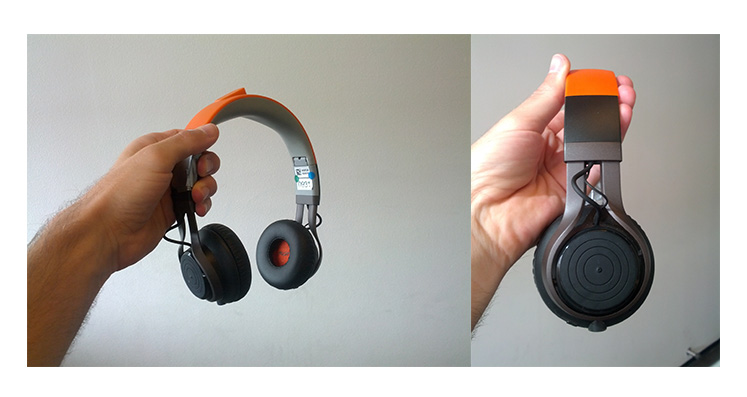
\includegraphics[width=0.9\textwidth,height=\textheight,keepaspectratio]{./Figures/headset.jpg}
		\rule{35em}{1pt}
	\caption[The Intelligent Headset]{The Intelligent Headset. A button is placed in the center of the left and right speaker (shown to the right).}
	\label{fig:headset}
\end{figure}

The headset features can be exploited through mobile applications using an included SDK targeting the iOS and Android platform (iOS SDK currently at version 1.82 and an Android SDK running verson 1.21 \footnote{Version information from 05-05-2014. Developer site: \url{https://developer.intelligentheadset.com/our-sdk/}}). The platform used in this project is Apples iOS. The main reason for using this platform is that when this project started the Intelligent Headset only provided an SDK compatible with iOS and still - though accessible for the Android platform today - the iOS SDK is running a higher version number making it more mature i.e. stable.

The SDK is implemented in the Spatial Music Menu application. The Intelligent Headset API (Application Programming Interface) provides features like reading the raw sensor data from all sensors, button events and functions for headset connectivity and 3D audio handling. An overview of the components and their communication is shown in figure \ref{fig:implementationoverview}.

\begin{figure}[t]
	\centering
		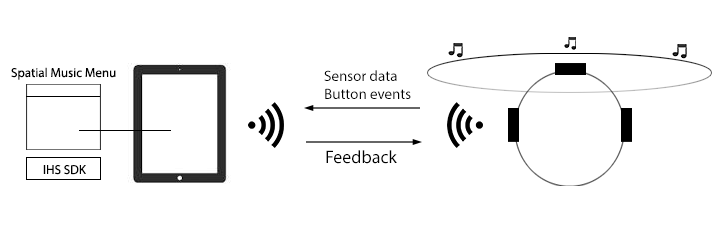
\includegraphics[width=0.9\textwidth,height=\textheight,keepaspectratio]{./Figures/implementation_overview.png}
		\rule{35em}{1pt}
	\caption[Implementation overview]{An overview of the components of the implementation and their communication}
	\label{fig:implementationoverview}
\end{figure}

\subsection{3D audio handling}
The combination of realtime sensor data and the IHS SDK functionality of setting specific audio items positions provided the required tools for implementing the audiospace. To place the audio items we used a 3D audio grid that served as a model for the audio listener and audio items, but also as a view mapping this audiospace. This 3D audio grid were defined with a virtual area size e.g. 100x100 meters.

To place audio items in a circular way we used simple geometry. We only needed the horizontal position the x and y positions of audio items were positioned by the parametric equation for a circle:

$x = cx + r * cos(a)$

$y = cy + r * sin(a)$

Where $r$ is the radius, $cx$,$cy$ the origin, and $a$ the angle from $0$ to $2\pi$ radians. Same equation were used for the audio listener position for the "carousel" zoom effect. The listeners direction were simply set by the yaw value from the gyroscope sensor data output which is the rotation value (in degrees) around the z axis. An illustration of this is showed in figure \ref{fig:circlepositions}.

\begin{figure}[t]
	\centering
		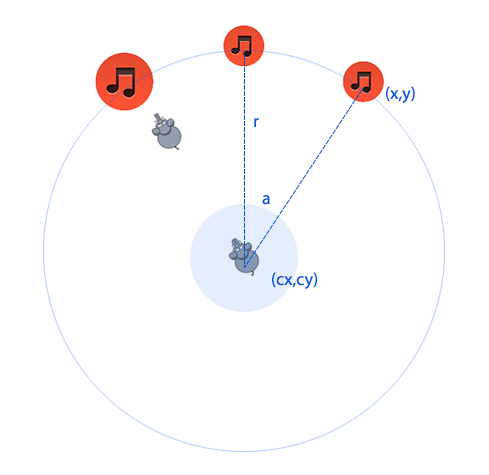
\includegraphics[width=0.6\textwidth,height=\textheight,keepaspectratio]{./Figures/circlepositions.png}
		\rule{35em}{1pt}
	\caption[Audio items positioning]{Listener and audio items positioning using circle equations.}
	\label{fig:circlepositions}
\end{figure}

\section{Music}
We used Deezer\footnote{\url{https://www.deezer.com/}} as a music provider in the implementation. Deezer is a music streaming service and provides an iOS SDK for accessing different kinds of information through their REST API e.g. track info, user playlists, albums, streaming urls, etc. This information is provided as JSON - a track item from a playlist could look like this:

\begin{lstlisting}
"tracks": {
    "data": [
      {
        "id": "1152226",
        "readable": true,
        "title": "Darkroom",
        "link": "http://www.deezer.com/track/1152226",
        "duration": "271",
        "preview": "http://cdn-preview-6.deezer.com/stream/6452dbcd46c90a70cb1147666ffd91ae-0.mp3",
        "artist": {
          "id": "1334",
          "name": "Archive",
          "link": "http://www.deezer.com/artist/1334",
          "tracklist": "https://api.deezer.com/artist/1334/top?limit=50",
          "type": "artist"
        },
        "album": {
          "id": "123427",
          "title": "Londinium",
          "cover": "https://api.deezer.com/album/123427/image",
          "tracklist": "https://api.deezer.com/album/123427/tracks",
          "type": "album"
        },
        "type": "track"
      },
\end{lstlisting}

A track represents an artist in the first level of the menu (HOME level) and by selecting a track (going up to ALBUM level) only tracks associated with the chosen tracks album id will appear. The final selection is simply the chosen album track (PLAYING TRACK level). The audio is provided by the "preview" urls which is pointing to 30 seconds preview clips. The fact that Deezer provides these preview clips of all their music was one of the main reason for using their services. This is very convinient as it is not possible to spatialise audio streams using the IHS SDK. Instead the IHS SDK is quite limited in that the only way to place sound sources in the spatial audio space is to use 16-bit wav format. Deezers preview tracks comes in MP3 format so every track needed conversion to 16-bit wav before use. 

All music information, download of preview tracks and conversion of audio was handled dynamically inside the Spatial Music Menu iOS application making it easier to add, remove and switch tracks. Basically one could add music tracks to the application by creating a Deezer playlist which is then synchronized by the iOS application. A synchronization operation is simply: 1) Getting and saving all track information from playlists including the preview tracks MP3 url; 2) download all MP3 tracks and save on device; 3) convert all tracks to 16-bit wav and save on device.


\section{Head Gestures Recognition}
To recognize head gestures we used DTW (Dynamic Time Warping) which is a well-known technique to find an optimal alignment between two time dependent sequences \cite{muller_dynamic_2007}. Due to the simple gestures (short sequences) defined in the system design we used a classic simple DTW although there exists several techniques for speeding up the algorithm \cite{muller_dynamic_2007,salvador_toward_2007,akl_accelerometer-based_2010}. 

Essentially the DTW algorithm works by compairing two sequences of length N and M. A sequence consists of observations and an observation is a set of accelerometer data from the headset. For each observation comparison a local cost is calculated and a cost matrix is created (using dynamic programming). If there exists a path (warping path) from point (1,1) to (N,M) in the cost matrix that has an overall cost that is less than a predefined cost, then there is a match. The local cost of an observation is calculated from the sum of the euclidean squared distances of each observation value. A squared euclidean distance places progressively greater weight on objects that are farther apart. The total cost is then simply the sum of all the observation distances.

A preview of such a sequence example could look like this:

\begin{lstlisting}
...
Observation: (
    "0.1245155",
    "-0.9570605",
    "0.02343822"
),
Observation: (
    "0.3266701",
    "-1.189489",
    "-0.1518601"
),
Observation: (
    "0.09228797",
    "-1.126988",
    "0.01416059"
)
...
\end{lstlisting}

The values are 3-axis accelerometer data (in order) x, y and z. An sensor observation occurs $\sim$ 30 times per second. To avoid overloading the device CPU by trying to recognise gestures for every new observation we only run the gesture recognizer for every 30 observations i.e. every second. All gesture sequences are below 100 observations so we used a window size of 100 for the testing sequence. I.e. every second the last 100 observations are tested for possible gestures.

\subsection{Training data}
Compaired with other long motion gestures e.g. running or climbing stairs, our head gestures were short events. For obtaining training data these gestures were recorded per event so a simple view containing a start/stop record button was implemented. Also to identify which class the gesture belonged to, the view had a list of labels with the specific gesture type that was to be chosen before recording the specific gesture.

The possible pause between pushing the start/stop recording button and the start or end of the actual gesture would cause some noise in the recorded data. To solve this we removed observations from the start of the recorded sequence until the difference between the start and the following observation were \textgreater 0.01. The same check was done with the end and its preceding observations. This noise cleaning was done after gestures were recorded (in memory) and the cleaned training data was saved to the device storage.


\section{iOS Application}
The Spatial Music Menu appliation were developed for an iPad Mini running iOS 7.1. As an overview and introduction of the iOS framework is out of this thesis scope - the interested reader is referred to Apples developer portal\footnote{\url{https://developer.apple.com/}} where a comprehensive documentation on the framework is available. Instead this section will focus on the application architecture, the design patterns and most the important functionality of the Spatial Music Menu.

An overview of the application architecture is shown in figure \ref{fig:apparchitecture}. The figure highlights the different relationships between application state, headset events handling, view (and audio) controller logic and persistency storage. The application aims to use iOS best practice design patterns provided by Apple\footnote{\url{https://developer.apple.com/library/ios/referencelibrary/GettingStarted/RoadMapiOS/DesignPatterns.html}} e.g. Model-View-Controller and delegation patterns.

\begin{figure}[t]
  \centering
    \includegraphics[width=\textwidth,height=\textheight,keepaspectratio]{./Figures/app-architecture.pdf}
    \rule{35em}{1pt}
  \caption[App architecture]{iOS app architecture overview}
  \label{fig:apparchitecture}
\end{figure}

\subsection{Application state management}
... Singleton approach

\subsection{Headset events handling}
...

\subsection{View controller logic}
- TODO: show screenshots of iPad 3 views

\subsection{Models and persistency storage}
...









 % Implementation

\lhead{\emph{Evaluation}}
\chapter{Evaluation}
\label{sec:evaluation}
To study whether the implemented Spatial Music Menu could compete with a touch and vision-based music player interface, we designed and conducted an experiment where users should perform mental and physical demanding tasks while interacting with the interfaces. This aimed to simulate the "biking while interacting with a music player" scenario.

\begin{figure}[h]
	\centering
		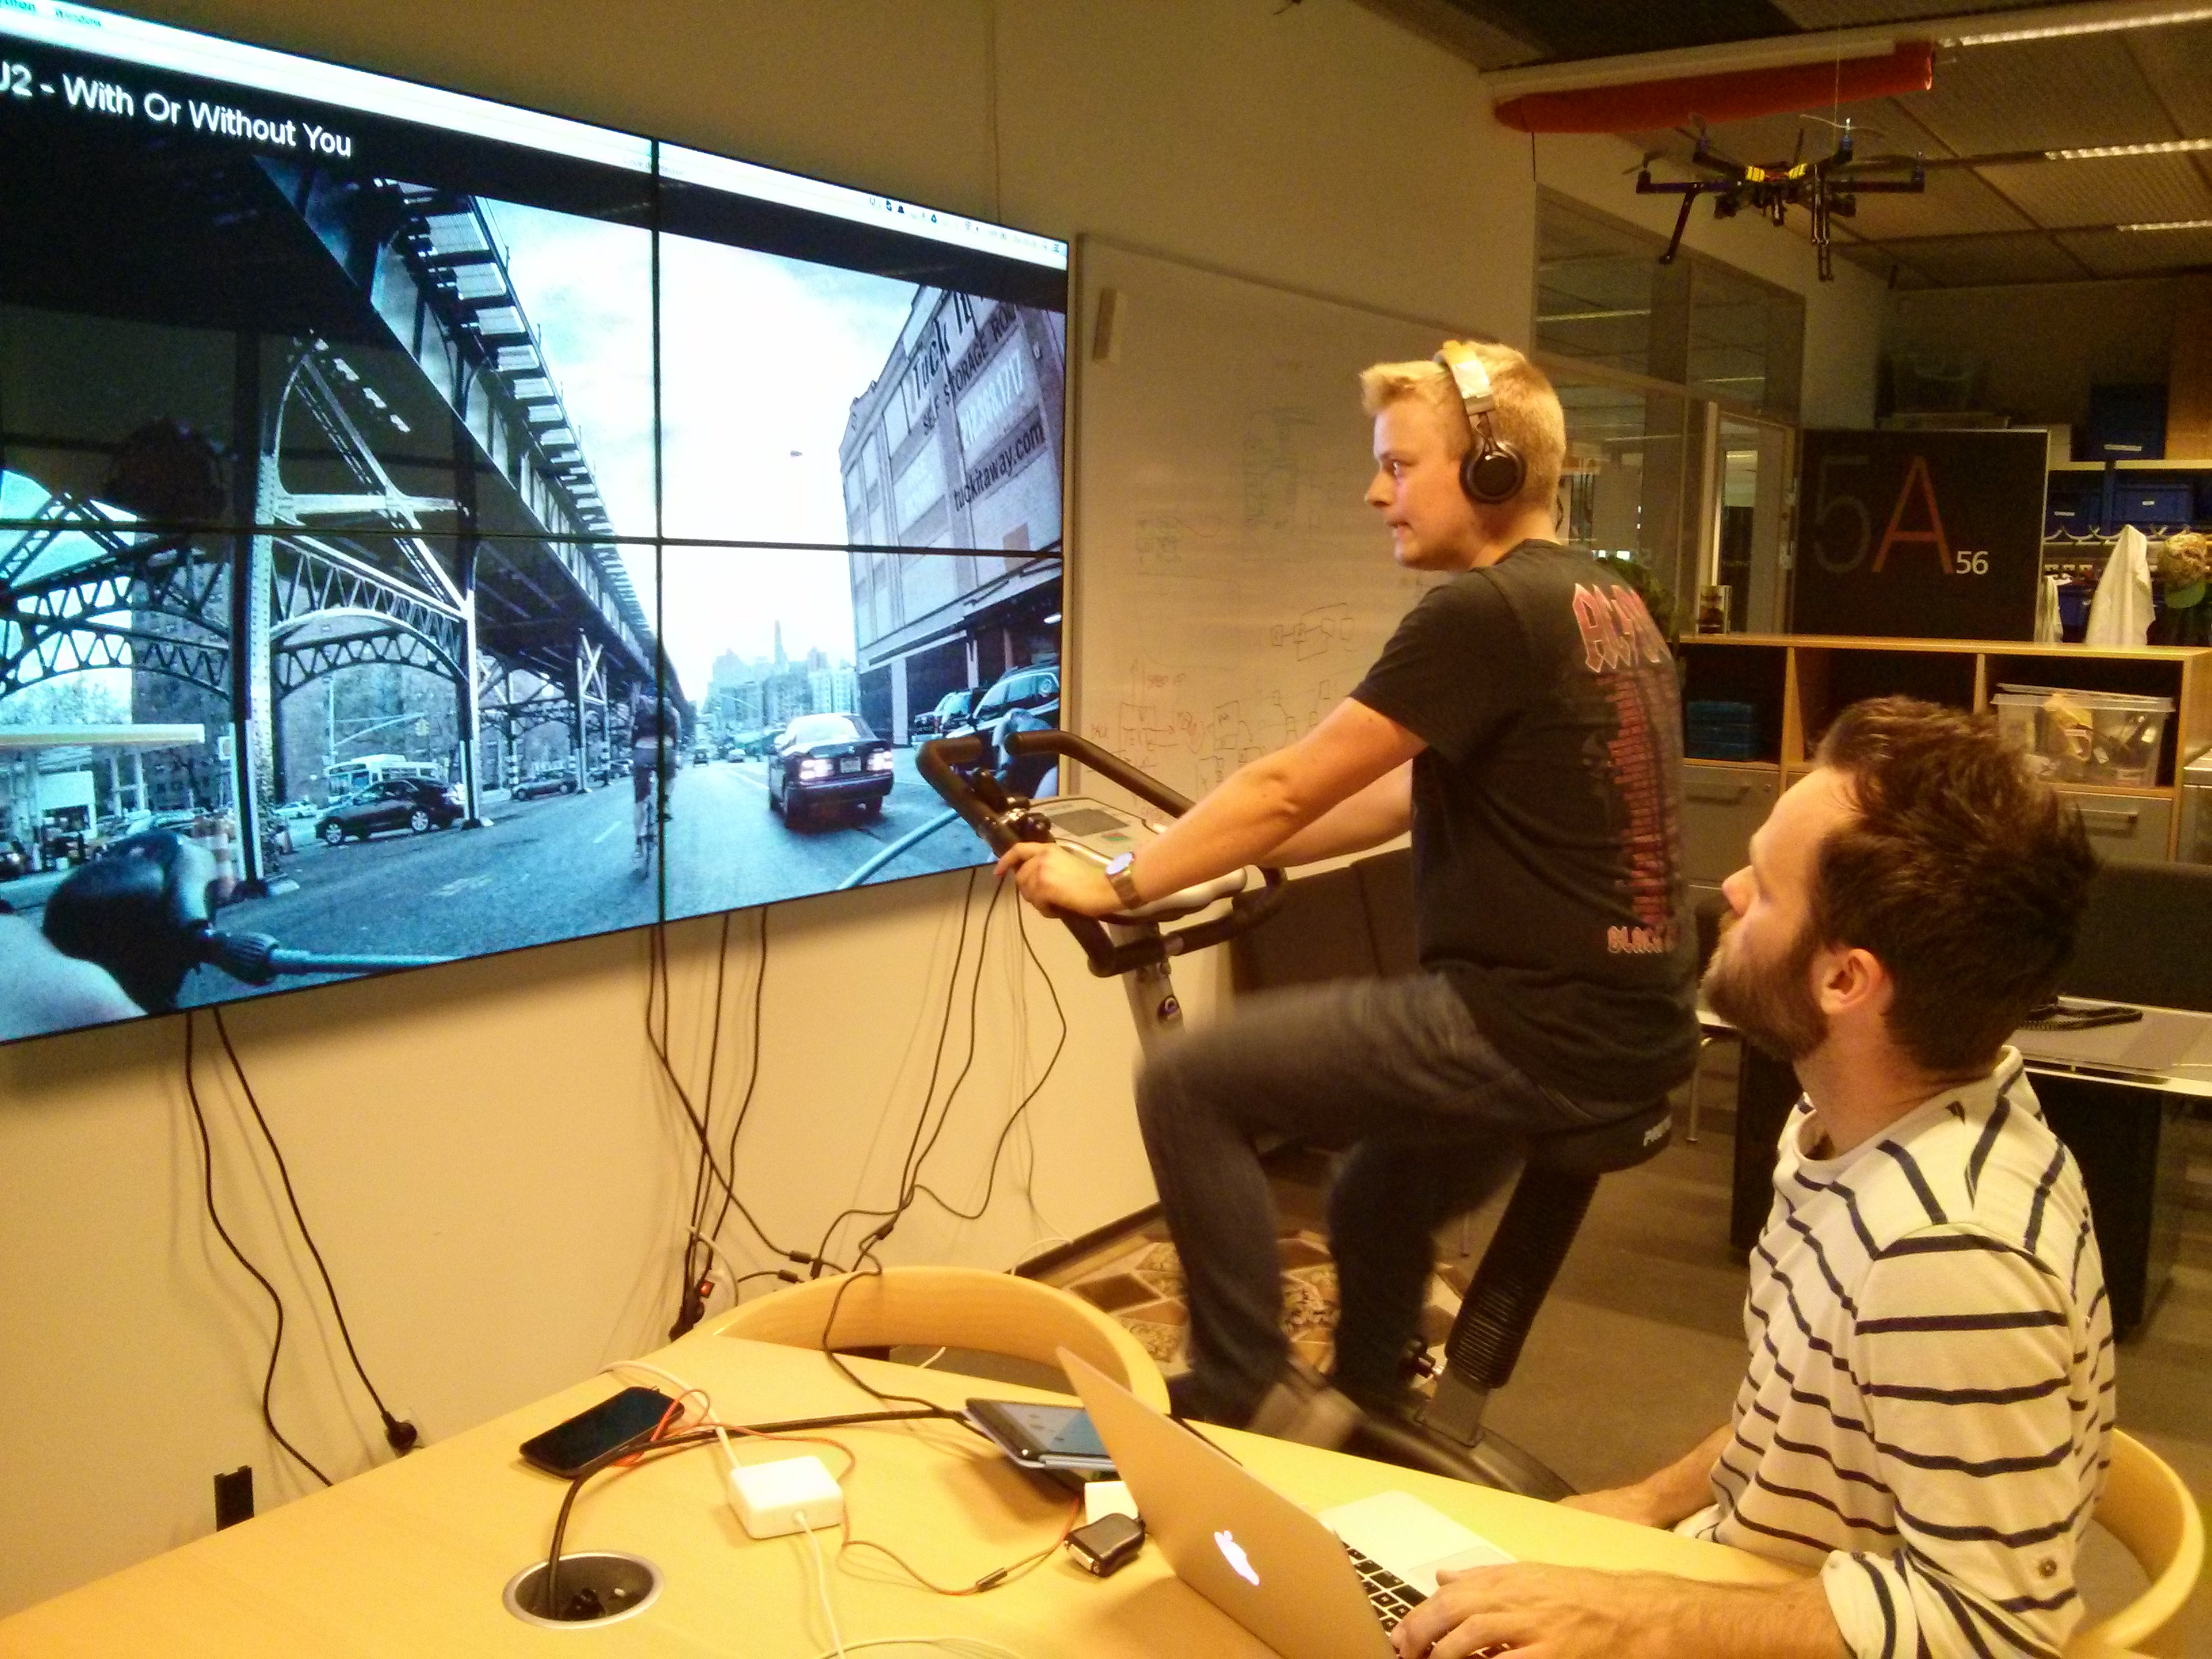
\includegraphics[width=0.7\textwidth,height=\textheight,keepaspectratio]{./Figures/evaluation_spatial.jpg}
		\rule{35em}{1pt}
	\caption[Evaluation Spatial Music Menu]{Participant performing a task using the Spatial Music Menu}
	\label{fig:evalspatial}
\end{figure}

% Scope
\textbf{Limitations and scope}

Although we in the explorative design process in \ref{sec:designsoundscape} evaluated that users could segregate 6-8 music tracks with the Spatial Music Menu, we reduced the number of tracks to 3 in this final experiment. An evaluation of the max number of simultanous playing music tracks while biking is out of this thesis scope and referred to a future study.

The participants used in the evaluation are acquaintances of us, so we are aware of the possibility that they might be biased in the sense that they want to "perform good". Throughout the experiment we tried to our best ability to be as objective as possible when explaining and instructing the systems.


\section{Experiment Design}
The experiment was designed and conducted as a controlled lab experiment. Controlled experiments are appropriate when comparing one design to another to see which is better \cite{benyon_designing_2010} and in this case we are compairing the Spatial Music Menu with a touch and vision-based music player. As the focus is on compairing and study the effects of these interfaces in an interaction in motion scenario i.e. biking, we designed an evaluation system simulating a trafficked biking scenario.

\subsection{Biking simulation}
A stationary bike was put in front of a giant screen (4 x 40 inch HD screens) that should simulate a road. To make the view as realistic as possible an image of an actual trafficked road\footnote{New York street: \url{http://timsklyarov.com/new-york-through-the-eyes-of-a-road-bicycle/}} was showed on the screen. To simulate obstacles that the user should be aware of or respond to in a real world biking scenario, 3 different shapes with random colors were displayed in random positions on the screen in a random time interval; between 0.3 and 1 second displaying the shape in 0.8 seconds. The shapes were circles, triangles and squares and the job for the person riding the bike was to detect the circles. This was done by pushing a button attached close to the users non-preferred hand on the steer, in this case a Playstation 3 joystick strapped with tape. The reason for the button placement at the non-preferred hand was, that the preferred hand should be used for navigating the touch and vision-based music player. To give the user feedback the circle was removed when detected. The screen simulation software is developed in Python 3 running on a Mac (OSX 10.9). The simulation system is illustrated in figure \ref{fig:simulationsystem}.

\begin{figure}[h]
	\centering
		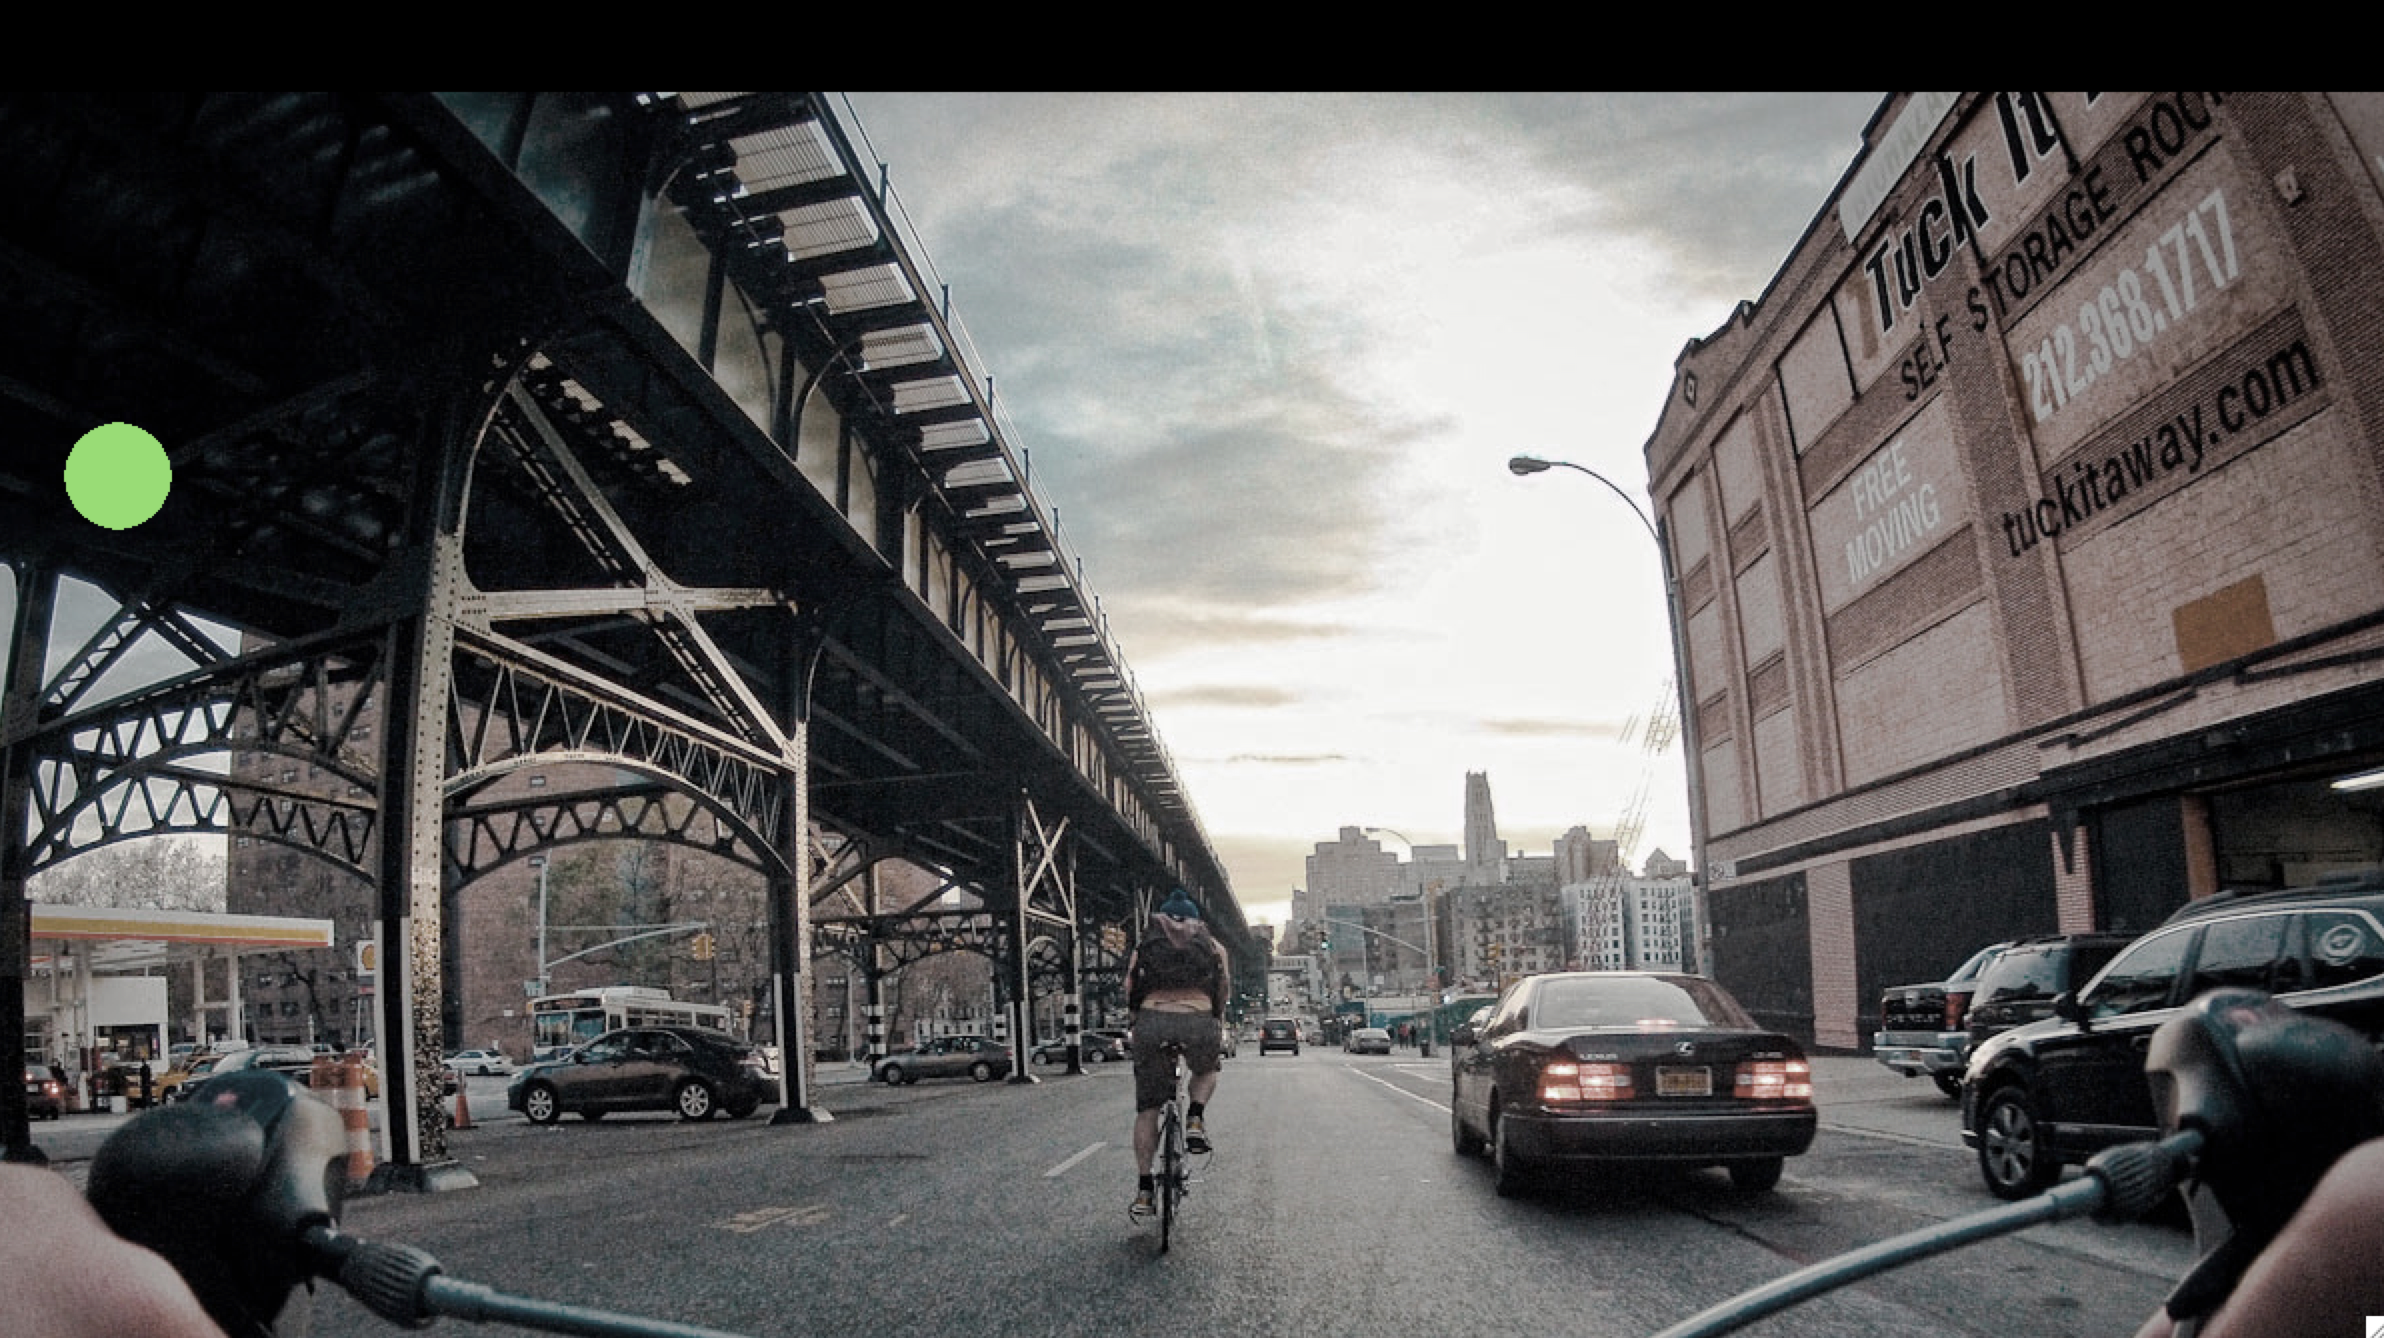
\includegraphics[width=0.6\textwidth,height=\textheight,keepaspectratio]{./Figures/simulation_system.png}
		\rule{35em}{1pt}
	\caption[Simulation screen]{The screen were to simulate a road and circles were obstacles that the user should respond to (detect) by pushing a button.}
	\label{fig:simulationsystem}
\end{figure}

\subsection{Touch and vision-based music player}
To represent a touch and vision-based music player we chose the music streaming service Deezer also used in the implementation (\ref{sec:implementationmusic}). Their Android application\footnote{\url{https://play.google.com/store/apps/details?id=deezer.android.app}} was installed on a Google Galaxy Nexus running Android 4.3. The same headset as for the Spatial Music Menu was used but this time connected through a wire.

\subsection{Hypotheses}
\label{sec:evaluationhypothesis}
Based on the related research theory and work laying ground for the design choices of the Spatial Music Menu, we derived the following hypotheses for the experiment:

\begin{description}
\item[Hypothesis 1:] The users ability to detect circles while executing tasks in the biking simulation will increase with the Spatial Music Menu interface compaired to the touch and vision-based music player interface.
\end{description}

\begin{description}
\item[Hypothesis 2:] The users performance when executing tasks in the biking simulation using the Spatial Music Menu can compete with the touch and vision-based music player interface in terms of general usability (workload) and task completion time.
\end{description}


\section{Method}
This section describes the different methods used for conducting the experiment.

\subsection{Participants}
5 persons (all male) were chosen for the evaluation. They all have in common that they listens to music while biking regularly. The participants had an average age of 30 years.

\subsection{System task}
Besides the task of detecting circles on the simulation screen the participants were given some tasks that refer to the system usage. Such a task is basically defined as a music track in which the user should navigate to. The music track (artist - title) is shown on the top left of the screen and when it does the user should start the navigation task. So in the case of the Spatial Music Menu the user should activate the menu by pushing the right button on the headset and explore and select the tracks with head gestures. If the user selects a wrong album or track the menu must be activated again (going to the HOME state). In the case of the Deezer music application the user must pick the device from a pocket, activate/unlock screen, navigate to the music track, deactivate screen and put the device back in the pocket.

As we wanted to compaire the two systems the menu structure needed to be aligned as much as possible. Figure \ref{fig:menustates} shows how the states (HOME and ALBUM) in the two different menus corresponds to each other.

\begin{figure}[t]
	\centering
		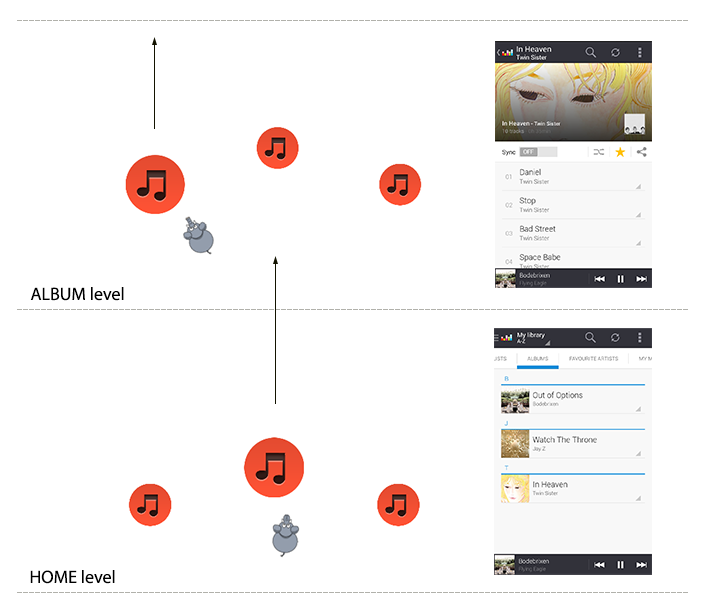
\includegraphics[width=0.9\textwidth,height=\textheight,keepaspectratio]{./Figures/menustates.png}
		\rule{35em}{1pt}
	\caption[Menu states comparison]{The HOME and ALBUM menu states definitions for each system.}
	\label{fig:menustates}
\end{figure}

The Deezer interface could imply an extra challenge in the ALBUM level, in that the entire album is showing on the screen compaired with the Spatial Music Menu where only 3 tracks appear per level. As an attempt to justify this we created an extra challenge in shuffling the 3 tracks on both levels in the Spatial Music Menu preventing the user to create a virtual map of the tracks. This would also enforce the spatialisation effect if users were still able to select and explore tracks efficiently.

\subsection{Procedure}
% Before test
As an intitial requirement for the experiment the participants had to select some of their favourite music tracks to be used in the systems - more specifically they had to choose 3 tracks from the same album for 3 different artists i.e. 9 tracks in total. The users were told that the music tracks should be very familiar e.g. hearing the song should trigger the artist name and song title.

Before starting the experiment the user were instructed in how the Spatial Music Menu works i.e. which head gestures to use for navigating and how the menu structure looks. They then got a chance to try out the system both standing still and while riding the stationary bike. In the standing still scenario the user was allowed to look at the menu envisioned on the iPad screen to get a sense of the menu structure and interaction feedback.

When the user felt ready the experiment started. The user started riding the bike and detecting the circles on the screen while listening to a chosen music track. While the gyroscope in the Intelligent Headset requires up to 10 seconds on application startup to calibrate we waited 10 seconds and then calibrated it again only this time with our system (aligning the center of the menu, described in \ref{sec:implementationviewsandcontrollers}). During the experiment 9 different system tasks were given to the user and when a task was done the user raised the right hand and a timestamp was registered in the simulation system (simple push of a button by the observer). The user were to detect circles at the same time throughout the experiment.

A user conducted this procedure for both the Spatial Music Menu and the Deezer music application and the order of which system was evaluated first were split so that 3 participants started with the Spatial Music Menu and 2 started with the Deezer application. Figure \ref{fig:evalspatial} and \ref{fig:evalnormal} shows a user performing a task using the Spatial Music Menu and the Deezer music player respectively.

\begin{figure}[t]
	\centering
		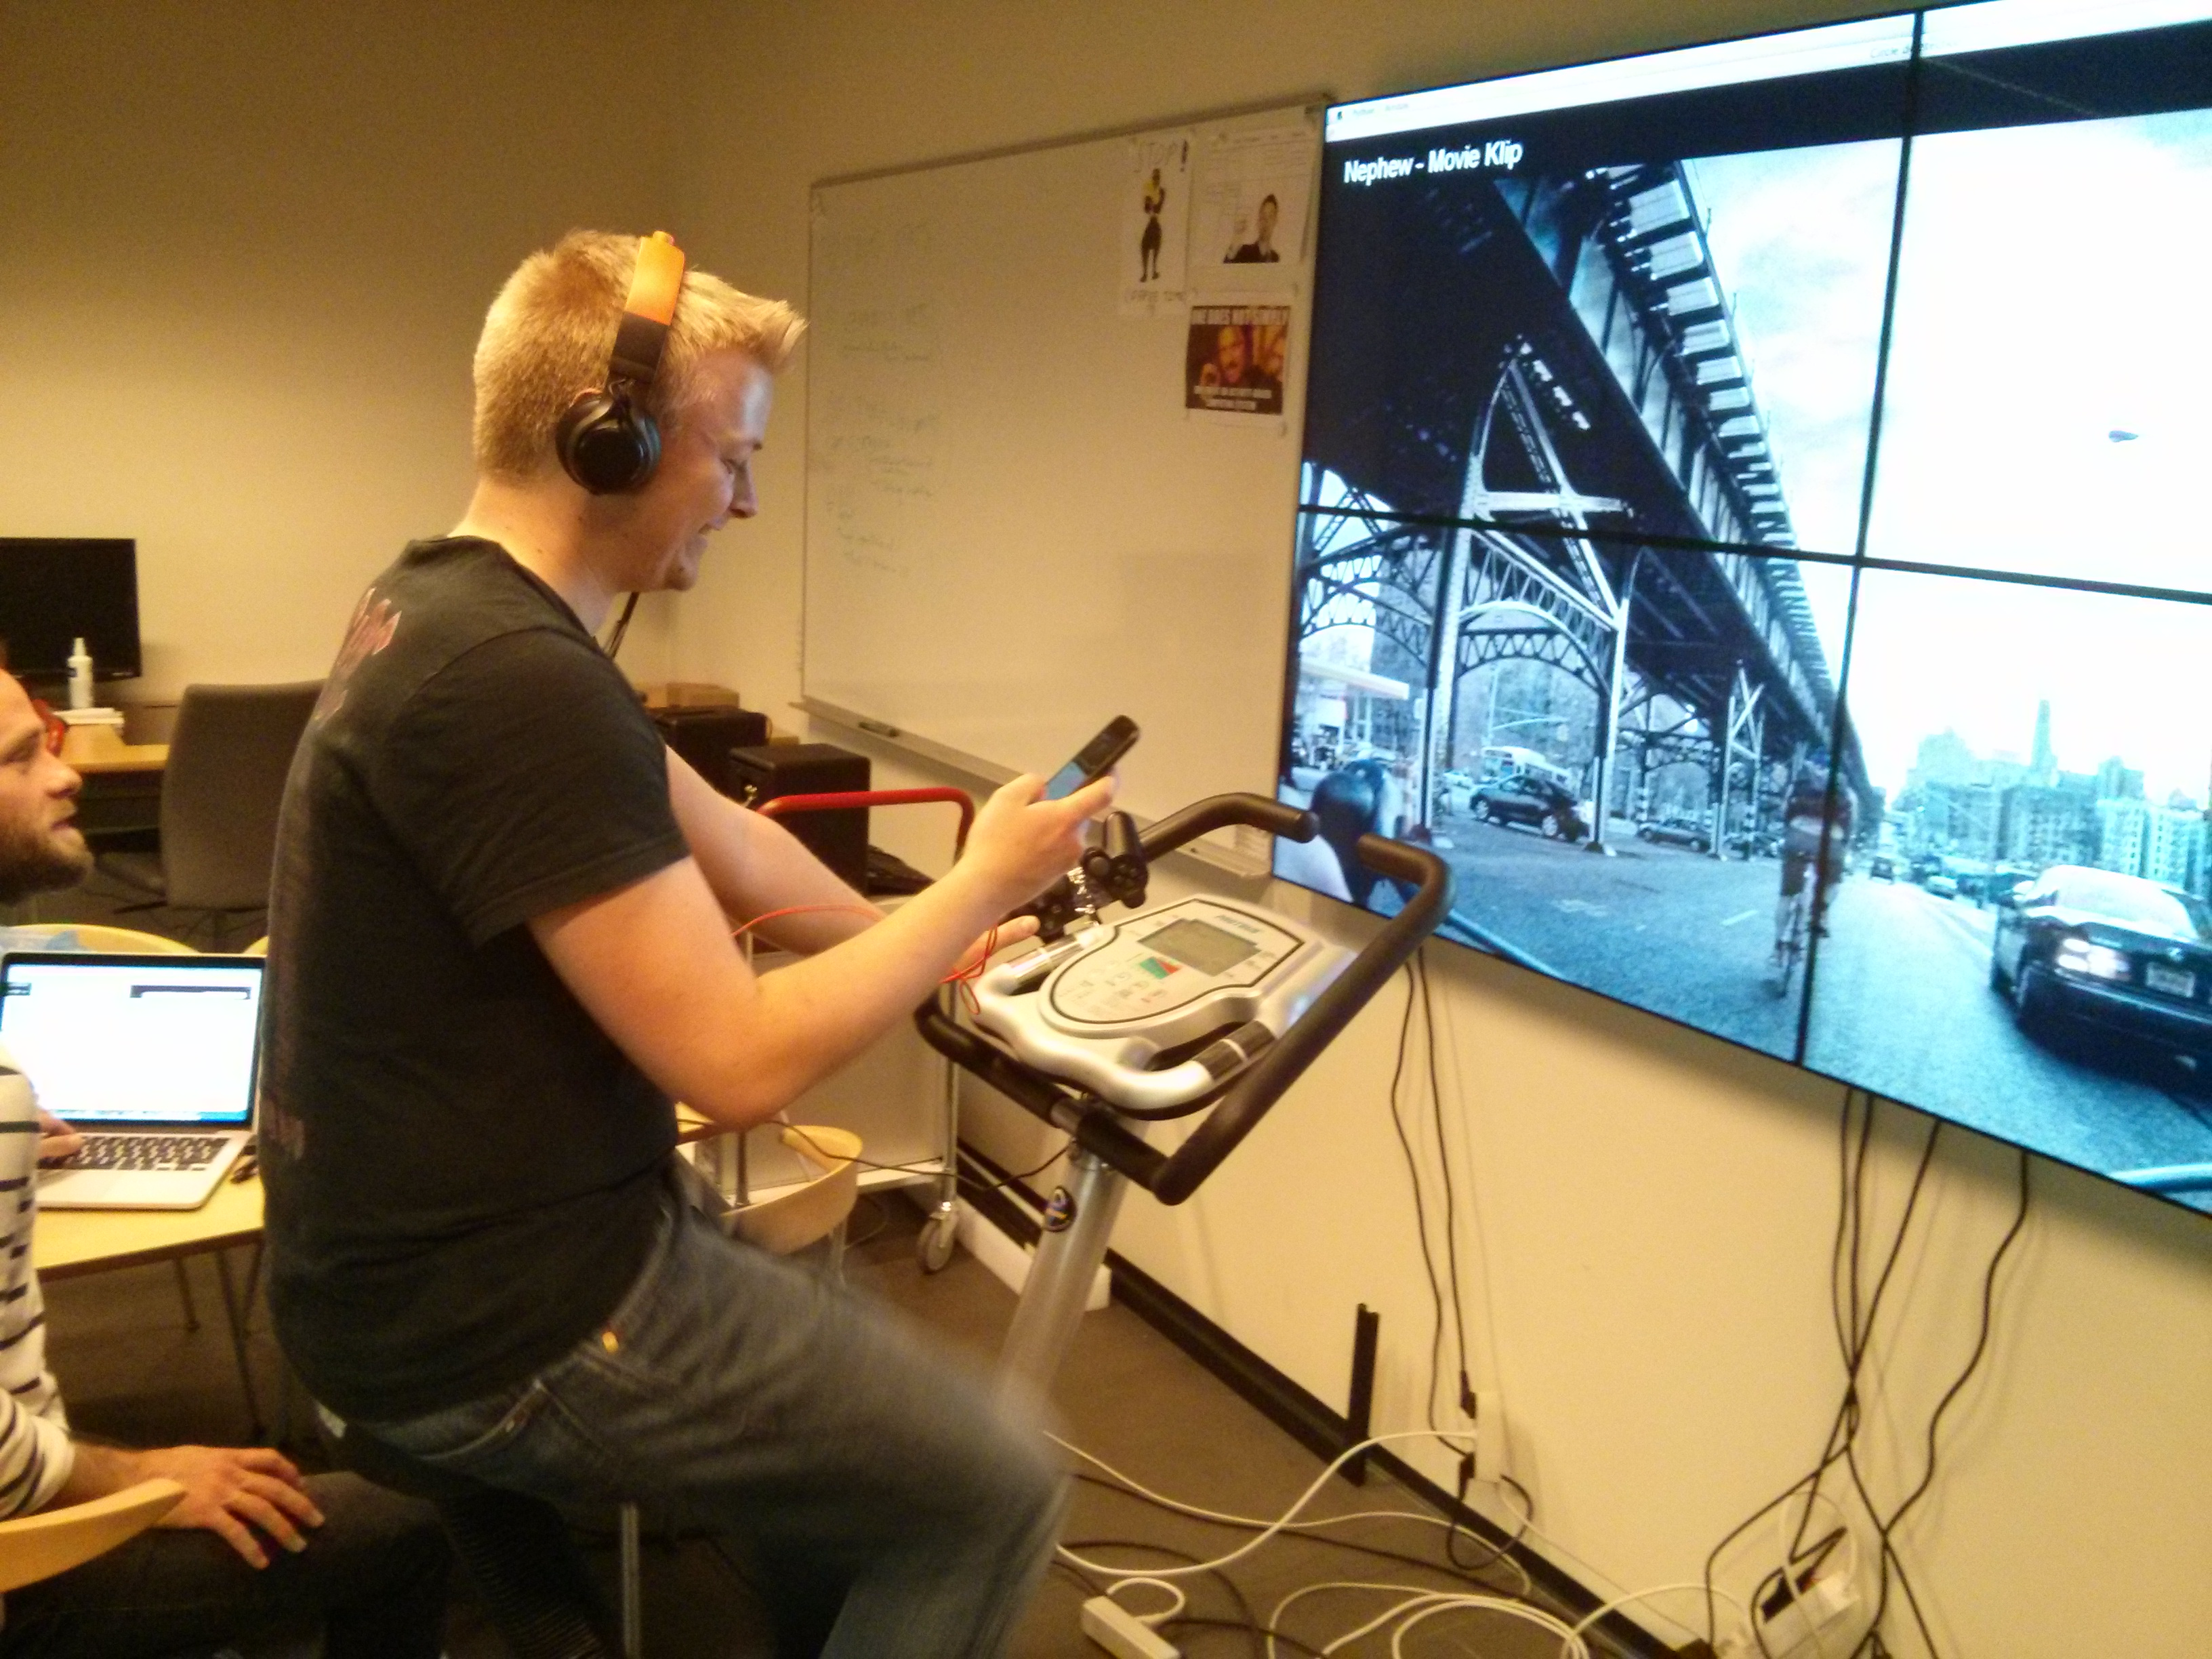
\includegraphics[width=0.7\textwidth,height=\textheight,keepaspectratio]{./Figures/evaluation_normal.jpg}
		\rule{35em}{1pt}
	\caption[Evaluation touch and vision-based interface]{Participant performing a task using a touch and vision-based music player}
	\label{fig:evalnormal}
\end{figure}

\subsection{Logging}
Throughout the experiment several data were logged. This includes data from the Biking Simulation System: Task start/end, circles shown, circles detections, error detections - and data from the Spatial Music Menu: Gestures detected, navigation steps including track info, headset connection status. Every log subject has a timestamp and as logging was performed on two different systems - iOS and OSX (python script) clocks were synchronized before comparison.


\subsection{NASA Task Load Index}
Subjective workload was measured using the NASA Task Load Index (TLX) scales \cite{hart_workload_1990}. The scales includes mental demand, physical demand, temporal demand, performance, effort and frustration in which each participant should rate after testing (Appendix \ref{sec:appendixnasatlx}). The user ratings gives a qualitative analysis of the system and the perceived workload is linked with the general usability of the system.

\subsection{Observation}
Participants were observed during the experiment to make sure they followed the instructions and to check and possibly prevent any kind of system obstruction. For example in between navigation tasks, when the user were listening to a selected track (PLAYING TRACK level), we made sure that the gyroscope was calibrated properly by compairing the direction on the iPad screen and the actual users head direction (using the calibrate button if neccesary, explained in \ref{sec:implementationviewsandcontrollers}). Also this observation gave us a chance to notice any particular repeating patterns in the way the users interacting with the systems, though we will not conclude anything from this in the results.


\section{Results}
This section presents the results of the experiment which were collected from logged data and the NASA TLX scales. Each participant did 9 tasks each, that is 45 tasks in total for each system and each participant filled out the NASA TLX scales for both systems.

\subsection{User attention}
We measured circle detection rate as an indicator of the users ability to attend to surroundings while interacting. The circle detection rate is the circles detected out of the circles shown during one task (in percent). Figure \ref{fig:resultscircles} shows the average rate for all 9 tasks for each participant using both systems.

\begin{figure}[h]
	\centering
		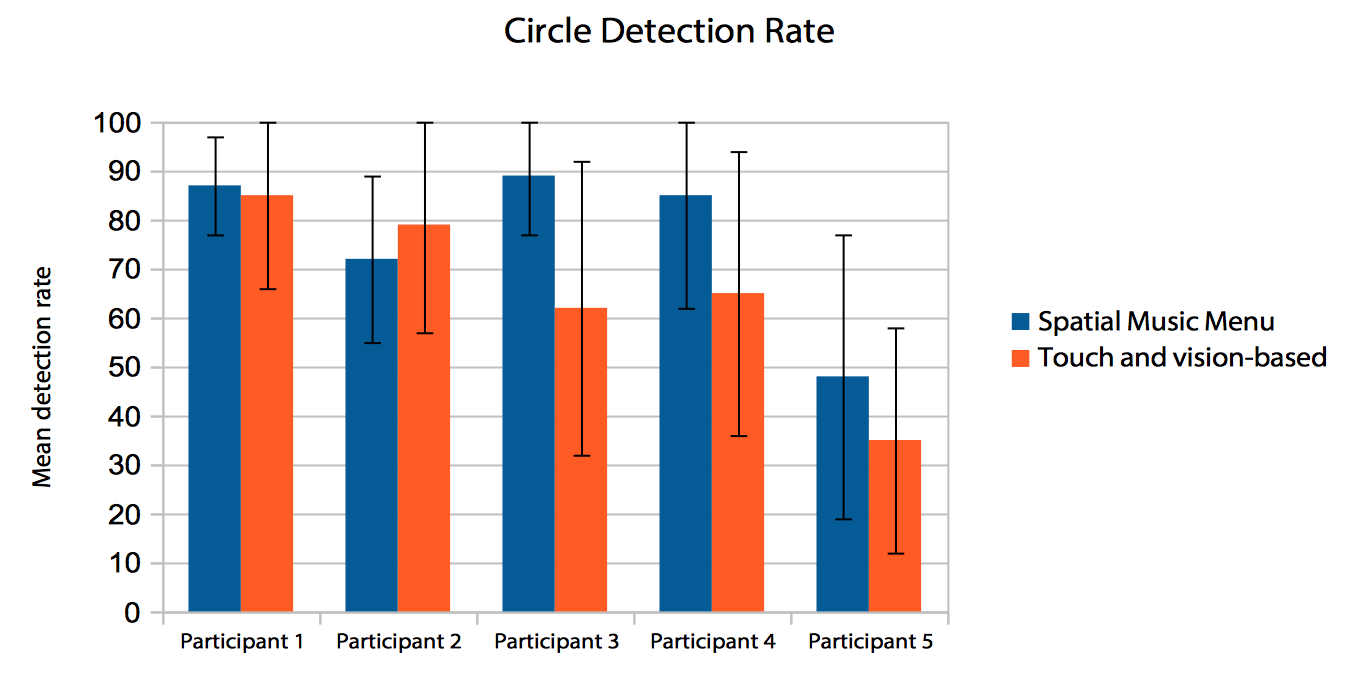
\includegraphics[width=0.9\textwidth,height=\textheight,keepaspectratio]{./Figures/results_circledetections.png}
		\rule{35em}{1pt}
	\caption[Results Circle Detection Rate]{Average circle detection rate for each participant}
	\label{fig:resultscircles}
\end{figure}

To verify \textit{Hypothesis 1} (page \pageref{sec:evaluationhypothesis}) we used a t-test to compaire circle detection rate between the two systems. The statistical test showed that there was a significant difference in the scores for the Spatial Music Menu (M=0.76) and the touch and vision-based music player (M=0.65) conditions; t(88)=1.66, p = 0.028 $<$ 0.05. In other words the circle detection rate is significantly higher when interacting with the Spatial Music Menu while biking.

\subsection{User performance}
Two measurements should give indications of the user performance. The first one is the task completion time - simply the time it took for a user to complete one task. Figure \ref{fig:resultstasktime} shows the average task completion time for all 9 tasks for each participant using both systems.

\begin{figure}[h]
	\centering
		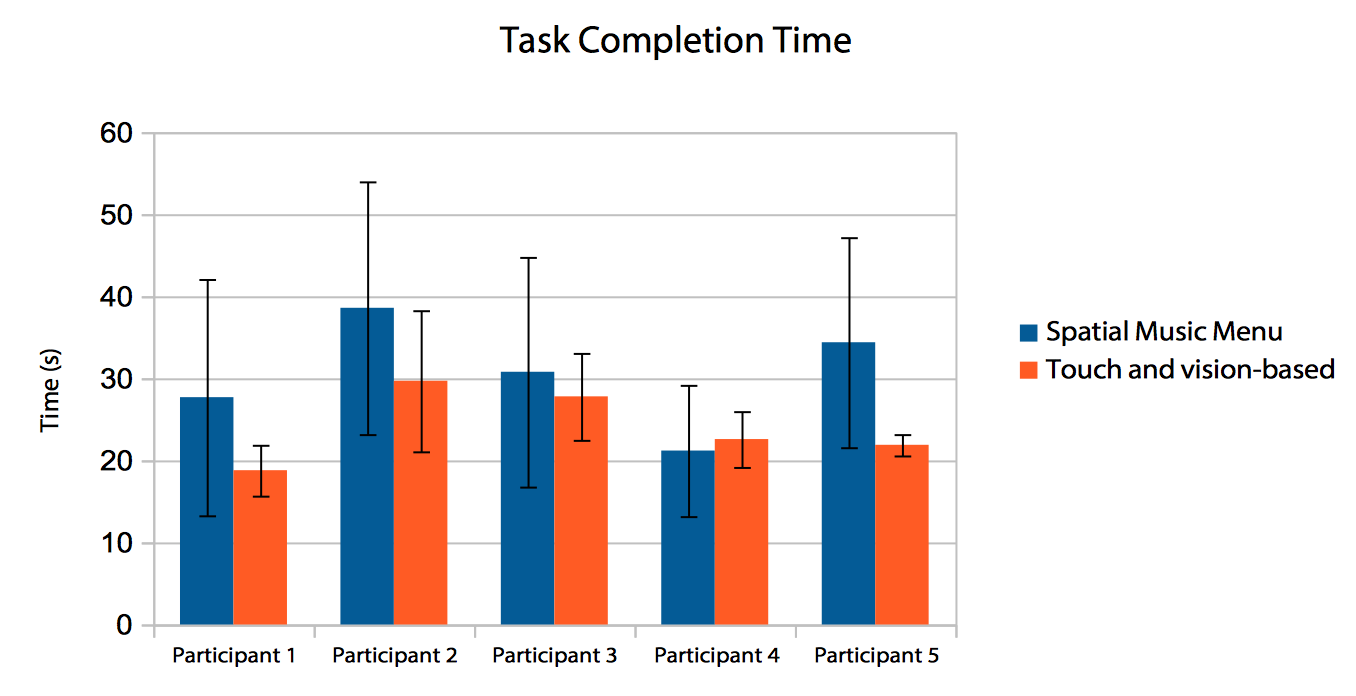
\includegraphics[width=0.9\textwidth,height=\textheight,keepaspectratio]{./Figures/results_tasktime.png}
		\rule{35em}{1pt}
	\caption[Results task time]{Time taken (in seconds) in average to execute a task for the participants.}
	\label{fig:resultstasktime}
\end{figure}

To verify \textit{Hypothesis 2} (page \pageref{sec:evaluationhypothesis}) in terms of task performance efficiency we used again a t-test to compaire the task completion time between the two systems. The statistical test showed that there was a significant difference in the scores for the Spatial Music Menu (M=30.53) and the touch and vision-based music player (M=24.13) conditions; t(88)=1.66, p = 0.003 $<$ 0.05. So in short the time it takes to complete a task, or navigate to a music track, is significantly higher in the Spatial Music Menu compaired to the touch and vision-based system.

To verify \textit{Hypothesis 2} in terms of the systems general usability we gathered qualitative data in form of participant ratings from the NASA TLX scales. The average of the participants scores for each of the 6 subscales are shown in figure \ref{fig:resultsnasatlx}.

\begin{figure}[h]
	\centering
		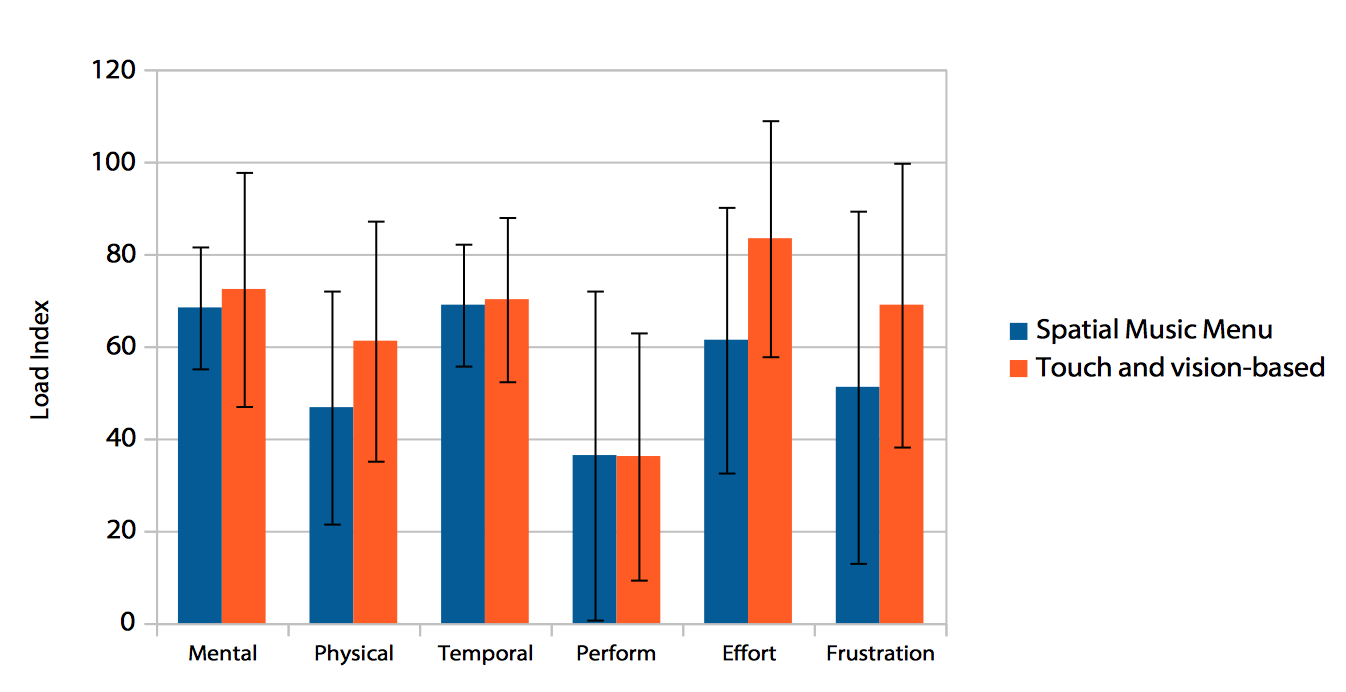
\includegraphics[width=0.9\textwidth,height=\textheight,keepaspectratio]{./Figures/results_taskloadindex.png}
		\rule{35em}{1pt}
	\caption[Results NASA TLX Score]{NASA TLX overall workload score for the participants (lower is better).}
	\label{fig:resultsnasatlx}
\end{figure}

The results show lower scores for the Spatial Music Menu in Physical Demand, Effort and Frustration while Mental Demand, Temporal Demand and Performance scores are more or less the same for both systems. The average of the participants total workload was 55.5 for the Spatial Music Menu and 65.4 for the touch and vision-based system.


\section{Discussion}
The results from the evaulation verified the first hypothesis, that participants were able to detect more circles interacting with the Spatial Music Menu comparied to the touch and vision-based. The main reason for this is that the visual focus can stay only on the screen (road) using the Spatial Music Menu while it is attending two visual tasks with the touch and vision-based system. It should be noted however that some participants during some tasks actually moved the eyes in the direction their head was pointing - however the chance of detecting a circle in the corner of the eye is still greater than when looking down on a screen.

The verification of the second hypothesis had mixed results. The task completion time for the Spatial Music Menu were significantly slower than the touch and vision-based system i.e. in terms of task performance efficiency the Spatial Music Menu could not compete with the touch and vision-based music player. If we look at figure \ref{fig:resultscircles} we notice a high spread for the Spatial Music Menu while the touch and vision-based system generally has a lower one making it more stable. However while the Spatial Music Menu shows that there exists challenges in that some tasks took a very long time to complete, it also shows a potential in that tasks can be performed very fast - faster than the touch and vision-based system.

However in terms of usability the Spatial Music Menu showed an overall lower workload score than the touch and vision-based music player. We are aware that these scores are only qualitative indications and that more than 5 participants could provide us with a more realistic picture.

\subsection{Challenges}
During the evaluation we observed a few challenges that could affect the results. First of all the headset gyroscope was a bit challenging in that it sometimes during execution of tasks "drifted" i.e. causing the menus center position moved a bit to the left/right. We did our best to calibrate the gyroscope in between tasks but this could affect a users task performance and workload.

Secondly some of the participants complained about some music tracks being higher in volume than others. This is due to the fact that the quality of music tracks provided by the Deezer music service variate.

TODO: shuffling tracks in spatial musicmenu maybe a greater challenge than the $>$ 3 album tracks, user can still create a virtual map

TODO: Spatial sound through headphones depend on the HRTF recorded and might not fit to all persons as the ear constructions are different (Brewster chapter 12 "Non-Speech Auditory Output" \cite{brewster_human-computer_2003})












% OLD
% Number of circles, safety
%The most important task for the user during testing is to detect as many circles as possible. The number of circles shown and the number of circles detected were logged during execution of tasks. This will give a quantitative analysis of whether the user is able to monitor the surroundings while interacting with the systems and contribute to the safety problem focus.

% System, track exploring
%For measuring the content (music track) exploring part of the Spatial Music Menu all navigation information were logged on the iPad. 

% System, task time

% Music genre type and quality made an impact

% the shuffling in the Spatial Music Menu is maybe making a to big difference (time), the user can still "map" tracks in the Deezer app though > 3 tracks. At the same time this enforces the spatial effect.

% Maybe comfort as a measurement?
%(Taken from Brewster article)
%The final measure taken was comfort. This was based around a new scale developed by Knight et al. [10] called the Comfort Rating Scale (CRS) which assesses various aspects to do with the comfort of a wearable device. For a device to be accepted and used it needs to be comfortable and people need to be happy to wear it. Using a range of 20- point rating scales similar to NASA TLX, CRS breaks com- fort into 6 categories: emotion, attachment, harm, perceived change, movement and anxiety. Knight et al. have used it to assess the comfort of two wearable devices they are building in their research group. Using this will allow us to find out more about the actual acceptability our systems.



 % Evaluation

\chapter{Conclusion}
... % Conclusion

%% ----------------------------------------------------------------
% Now begin the Appendices, including them as separate files

\addtocontents{toc}{\vspace{2em}} % Add a gap in the Contents, for aesthetics

\appendix % Cue to tell LaTeX that the following 'chapters' are Appendices

\chapter{An Appendix}

Lorem ipsum dolor sit amet, consectetur adipiscing elit. Vivamus at pulvinar nisi. Phasellus hendrerit, diam placerat interdum iaculis, mauris justo cursus risus, in viverra purus eros at ligula. Ut metus justo, consequat a tristique posuere, laoreet nec nibh. Etiam et scelerisque mauris. Phasellus vel massa magna. Ut non neque id tortor pharetra bibendum vitae sit amet nisi. Duis nec quam quam, sed euismod justo. Pellentesque eu tellus vitae ante tempus malesuada. Nunc accumsan, quam in congue consequat, lectus lectus dapibus erat, id aliquet urna neque at massa. Nulla facilisi. Morbi ullamcorper eleifend posuere. Donec libero leo, faucibus nec bibendum at, mattis et urna. Proin consectetur, nunc ut imperdiet lobortis, magna neque tincidunt lectus, id iaculis nisi justo id nibh. Pellentesque vel sem in erat vulputate faucibus molestie ut lorem.

Quisque tristique urna in lorem laoreet at laoreet quam congue. Donec dolor turpis, blandit non imperdiet aliquet, blandit et felis. In lorem nisi, pretium sit amet vestibulum sed, tempus et sem. Proin non ante turpis. Nulla imperdiet fringilla convallis. Vivamus vel bibendum nisl. Pellentesque justo lectus, molestie vel luctus sed, lobortis in libero. Nulla facilisi. Aliquam erat volutpat. Suspendisse vitae nunc nunc. Sed aliquet est suscipit sapien rhoncus non adipiscing nibh consequat. Aliquam metus urna, faucibus eu vulputate non, luctus eu justo.

Donec urna leo, vulputate vitae porta eu, vehicula blandit libero. Phasellus eget massa et leo condimentum mollis. Nullam molestie, justo at pellentesque vulputate, sapien velit ornare diam, nec gravida lacus augue non diam. Integer mattis lacus id libero ultrices sit amet mollis neque molestie. Integer ut leo eget mi volutpat congue. Vivamus sodales, turpis id venenatis placerat, tellus purus adipiscing magna, eu aliquam nibh dolor id nibh. Pellentesque habitant morbi tristique senectus et netus et malesuada fames ac turpis egestas. Sed cursus convallis quam nec vehicula. Sed vulputate neque eget odio fringilla ac sodales urna feugiat.

Phasellus nisi quam, volutpat non ullamcorper eget, congue fringilla leo. Cras et erat et nibh placerat commodo id ornare est. Nulla facilisi. Aenean pulvinar scelerisque eros eget interdum. Nunc pulvinar magna ut felis varius in hendrerit dolor accumsan. Nunc pellentesque magna quis magna bibendum non laoreet erat tincidunt. Nulla facilisi.

Duis eget massa sem, gravida interdum ipsum. Nulla nunc nisl, hendrerit sit amet commodo vel, varius id tellus. Lorem ipsum dolor sit amet, consectetur adipiscing elit. Nunc ac dolor est. Suspendisse ultrices tincidunt metus eget accumsan. Nullam facilisis, justo vitae convallis sollicitudin, eros augue malesuada metus, nec sagittis diam nibh ut sapien. Duis blandit lectus vitae lorem aliquam nec euismod nisi volutpat. Vestibulum ornare dictum tortor, at faucibus justo tempor non. Nulla facilisi. Cras non massa nunc, eget euismod purus. Nunc metus ipsum, euismod a consectetur vel, hendrerit nec nunc.	% Appendix Title

\chapter{iOS Application Screenshots}
\label{sec:appendixviews}

\section{AudioMenu}

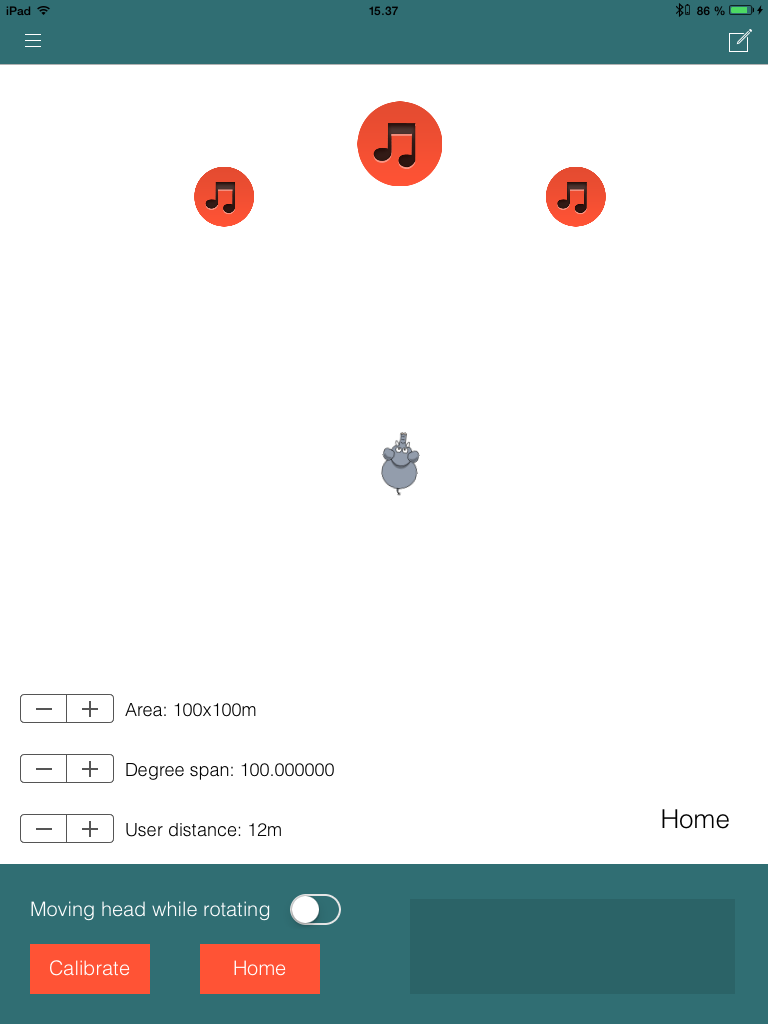
\includegraphics[width=0.7\textwidth]{Figures/view_audiomenu.png}


\section{Music}

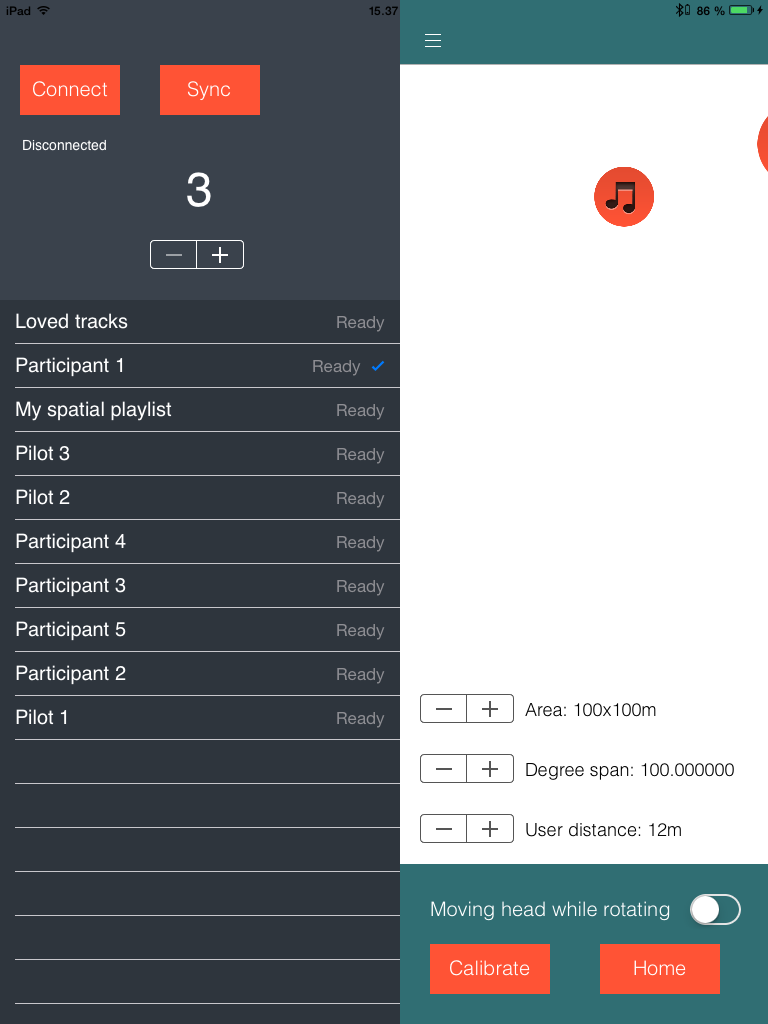
\includegraphics[width=0.7\textwidth]{Figures/view_music.png}


\section{Gestures}

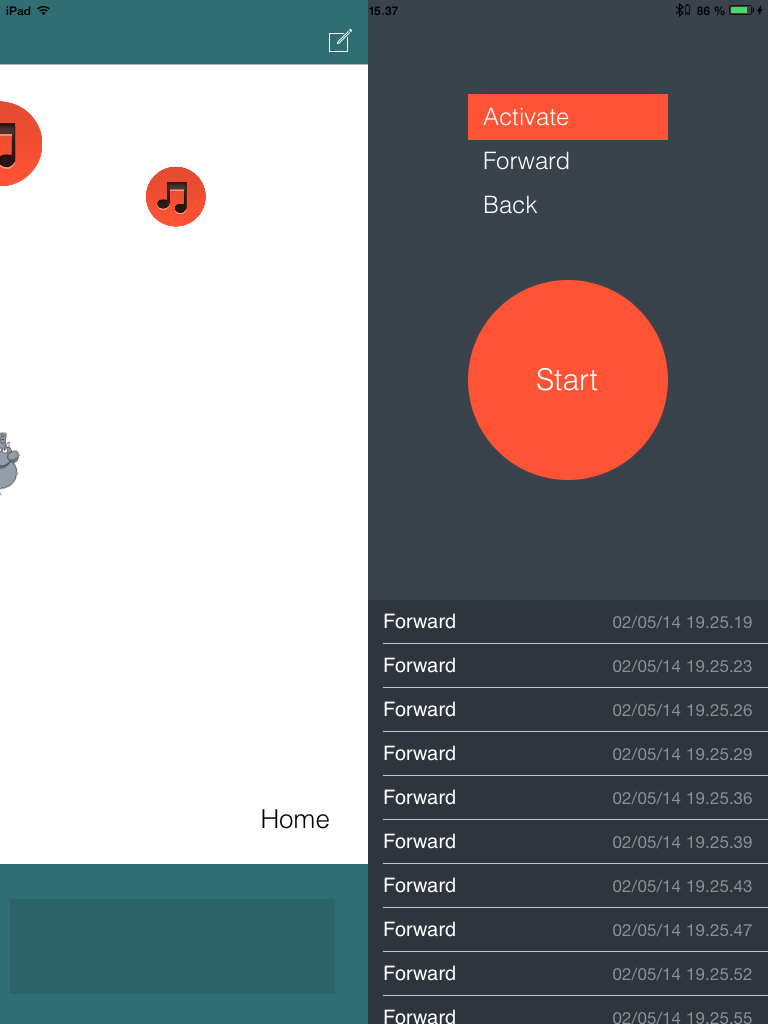
\includegraphics[width=0.7\textwidth]{Figures/view_gestures.png}



 % Appendix Title

\chapter{Software}

\section{iOS Application}
\label{sec:appendixios}
The iOS application is on github an can be cloned from: \url{https://github.com/johin/Thesis/tree/master/Application/SpatialMusicMenu}.


\section{Python Biking Simuation System}
\label{sec:appendixpython}
The Python Biking Simulation System (1 script) is on github an can be cloned from: \url{https://github.com/johin/Thesis/tree/master/Evaluation}. % Appendix Title

\addtocontents{toc}{\vspace{2em}}  % Add a gap in the Contents, for aesthetics
\backmatter

%% ----------------------------------------------------------------
\label{Bibliography}
\lhead{\emph{Bibliography}}  % Change the left side page header to "Bibliography"
\bibliographystyle{acm-sigchi}  % Use the "unsrtnat" BibTeX style for formatting the Bibliography
\bibliography{Bibliography}  % The references (bibliography) information are stored in the file named "Bibliography.bib"

\end{document}  % The End
%% ----------------------------------------------------------------